\documentclass[12pt]{revtex4}
\usepackage{ulem}
\usepackage{url}
\usepackage{epsfig}
\usepackage{graphicx,color}% Include figure files
%\usepackage{epstopdf}
\DeclareGraphicsRule{.tif}{png}{.png}{`convert #1 `basename #1 .tif`.png}
\usepackage[psamsfonts]{amssymb}
\usepackage{amsmath}
\usepackage{indentfirst}
%\usepackage{cite}

\usepackage{xcolor}

\newcommand{\be}{\begin{equation}}
\newcommand{\ee}{\end{equation}}
\newcommand{\ba}{\begin{eqnarray}}
\newcommand{\ea}{\end{eqnarray}}

\begin{document}
%\title{Patterns of Human Learning in Complex Systems}
\title{Do modern humans solve problems with algorithms used by hunter-gatherers in search for food?}

\author{Thomas Maillart}
\email{thomas.maillart@unige.ch}
\affiliation{University of Geneva, Geneva, Switzerland}

\author{Johannes Castner}
\email{johannes@collectiwise.com}
\affiliation{University of Columbia, New York, United States of America}


\date{\today}


\begin{abstract}
%\vspace{1cm}
Recent research \cite{baronchelli2013levy} has suggested that cognitive mental search patterns \cite{rhodes2007human,radicchi2012rationality,radicchi2012evolution} may be inherited from typical foraging and mobility patterns of animals \cite{viswanathan1996levy,ramos2004levy,reynolds2007displaced} and humans \cite{gonzalez2008understanding,song2010mode\
lling,rhee2011levy}. In particular, patterns suggest that cognitive processes in abstract spaces are similar to food search algorithms of hunter-gatherers, modeled as L\'evy flights \cite{brown2007levy,raichlen2014evidence}. Here, we study the mental search trajectories of
individuals who have been asked to reverse engineer the conditional probabilities of 3-variable and 4-variable stochastic processes, as Bayesian
networks (48 participants per treatment) \cite{steyvers2003inferring,pearl2009causality}. We find an important contrast with the random trajectories predicted by L\'evy flight and random walk models, optimized for search of sparse targets %\cite{viswanathan1999optimizing,edwards2007revisiting,song2010modelling\
,viswanathan2011physics}.  
Human mental search exhibits temporal and spatial regularity, characterized by a time dependent distance between two consecutive solutions proposed by each individual.  Additionally, we find an unexpected tendency to return to previously tested solutions.  Both, contribute to a sub-optimal exploration of the
problem space, which in turn slows the speed of approaching the target solution.  Our results
suggest that inherent cognitive limitations hinder efficient exploration of complex abstract spaces.  These limitations appear to be hard-wired in our brain, and may stem from previously evolutionary fit hunting strategies that are inefficient for solving hard problems in modern environments. 

\end{abstract}

\maketitle

\section{Introduction}
In scientific research \cite{}, software engineering and cybersecurity \cite{}, politics \cite{}, and daily life \cite{}, individuals face problems that involve many interdependent variables and thus large problem spaces, although only sparse -- or unique -- solutions exist \cite{}. These problems are known to be hard to humans, and have been studied by cognitive scientists \cite{Neurath's boat}. In cognitive science, reverse-engineering a Bayesian Network, which involves complicated interdependencies, has become a typical way to probe cognitive capabilities \cite{}. Because variables are dependent, landscapes are not smooth and solutions cannot be reached by simple local search/optimisation strategies {\bf (could we illustrate this point in a way or another with a figure?)}. 

Here, we investigate the fine-grained cognitive mechanisms of complicated problem resolution, which involves 2 treatments {\bf for} the resolution of 3-node and 4-node Bayesian networks over one trial of XX minutes, with a warm-up period of YY. Reverse-engineering these Bayesian networks involve evaluating respectively 8 and 16 conditional probabilities (varying from $0$ to $1$). Any change to any of these probabilities is registered with a resolution of one second [see Supplementary Information (SI) \ref{SI_experiment}]. On average, participants perform poorly in both treatments (see Figure \ref{fig:1}A), and improvement of the proposed models over time follows an extremely slow decay [with Jensen-Shannon Distance $D_{jsd}(t) \sim t^{\nu}$ with $ \nu \approx -0.15(1)$]. 

\begin{figure}[h!]
\begin{center}
\includegraphics[width=17cm]{figures/figure1.eps}
\caption{\footnotesize{{\bf A.} Average Euclidian Distance $\langle D \rangle$ decays as function of time as $\sim t^{\nu}$ with $ \nu \approx -0.15(1)$ indicating a very slow convergence to the true model {\bf [indicate $t_0$s and what their values may mean]}. {\bf B.} Probability density function of displacement $pdf(\Delta r) = \Delta r^{-\alpha -1}$ with $\alpha = 0.40(5)$ with a cut-off limited by the largest possible displacement, which is $\sqrt{k}$ with $k$ the number of conditional probabilities to evaluate. {\bf C.}  Probability density function of waiting time $\Delta t$ $pdf(\Delta t) = \Delta t^{-\beta -1}$ with 2 regimes : $\beta_{\Delta t < 125} = 0.38(4)$ and $\beta_{\Delta t > 125} = 1.59(5)$. Distributions of $\Delta r$ and $\Delta t$ are equivalent for the simple and complex treatments.}}
\label{fig:1}
\end{center}
\end{figure}

Humans -- like many other animals \cite{} -- use efficient strategies to search for food over large areas \cite{rhodes2007human}. These L\'evy walks strategies alternate many small local displacements and few long range displacement. Namely, the distribution of displacements obeys a power law: 

\begin{equation}
\label{displacements}
pdf(\Delta r) = \Delta r^{-\alpha -1}.
\end{equation}

We find that displacements between proposed models (on average over all participants) follow a similar power law distribution with $\alpha = 0.40(5)$ (see Figure \ref{fig:1}B). In addition, the distribution of waiting times $\Delta t$ between two iterations of model propositions, also follows a power law: 

\begin{equation}
\label{wtimes}
pdf(\Delta t) = \Delta t^{-\beta -1},
\end{equation}

with 2 regimes : $\beta_{\Delta t < 125} = 0.38(4)$ and $\beta_{\Delta t > 125} = 1.59(5)$. Distributions of $\Delta r$ and $\Delta t$ are equivalent for the simple and complex treatments. Together, equations \ref{displacements} and \ref{wtimes} define a Continuous Time Random Walk (CTRW) \cite{}, which is another flavour of food search for {\bf XXXanimals} in ecological systems \cite{book_ecological_systems}. The observed displacement exponent is significantly smaller, compared to optimal L\'evy walks of food search in ecosystems, typically found close to  $\alpha = 1$ \cite{} and mathematically optimal for search of sparse solutions in wide areas, provided that search is a memoryless process \cite{viswanathan1999optimizing, edwards2007revisiting,song2010modelling,viswanathan2011physics}. \\

\subsection{Memory in L\'evy Walks/Flights}

However, humans exhibit repeated behaviours, which imply memory. For instance, evidence from online auctions \cite{radicchi2012rationality}  suggests that optimal search strategy ($\alpha = 2 $) can be reached by humans when considering evolutionary forces \cite{radicchi2012evolution}. Sedentary human mobility (e.g., in cities) also exhibits repeated travel behaviours, such as between home and work places, with short displacements around few areas of particular interests, and with punctual travels beyond the borders of the city, e.g., to another city or country \cite{brockmann2006scaling,gonzalez2008understanding,song2010modelling}. Using mobile phone traces, Song et al.  have proposed a modified version of L\'evy flights, by incorporating a form of preferential attachment, which predicts that most visited places tend get even more visits \footnote{The model proposed by Song et al. \cite{song2010modelling} is however a challenge to common sense logic: Most visited places (i.e., home and workplace) are visited at a stable rate, roughly following circadian periods.}. Yet, on the contrary to early models \cite{viswanathan1999optimizing, edwards2007revisiting,song2010modelling,viswanathan2011physics}, proposed explanations by Radicchi et al. \cite{radicchi2012evolution} and Song et al. \cite{song2010modelling} incorporate memory, either through evolutionary forces to optimise online auction strategies (through {\it try and fails}), or human memory driving routine repeated visits of same places \cite{gonzalez2008understanding,song2010modelling}, because they bring renewal resources (mainly financial resources are derived from staying at work, while home may bring e.g., a roof for the night, rest and intrinsic rewards). {\bf Although we have not found documented evidence of memory for animals and nomad humans (such as e.g., hunter gatherers), they may similarly perform L\'evy flights with memory, returning to previously visited food spots, which have replenished between two visits [$\rightarrow$ is there a chance to find evidence for this, even if it's qualitative? I am really surprised this has not been documented yet.]}.\\

%\ref{fig:3}A ???


\subsection{An experiment to probe cognitive mechanisms involved for solving hard problems}

Hard problems {\bf [provide a strict definition of hard problems above, as much as possible, or refine terminology]} have a unique best solution, which can be approached. yet getting close to this solution is hard, because many interdependent variables are involved. 

Individuals tackling hard problems face a tension between testing and updating their beliefs from information stored in their memory (i.e., {\it exploitation} or {\it recombination of information}), and taking action to {\it explore} and update their belief from not previously available {\it exogenous} information. Taking such action would equivalent to the exploration of unknown territories by pioneers in the physical world. The former {\it exploitation} approach may bring improvement toward the solution, however limited to a {\bf (linear?) combination} of previously tried solutions. The latter approach is a {\bf more} high-risk high-return strategy, but whether it brings improvement towards the solution or not, it matters little, as this strategy primarily expands the {\bf convex hull of the explored portion of the solution space [not sure if we can say it this way]}. Once a new portion of the solution space has been explored, the attempted proposed model is then stored into memory and may be recombined, later on, with other proposed models. \\
\begin{figure}[h!]
\begin{center}
\includegraphics[width=12cm]{figures/figure2.eps}
\caption{\footnotesize{Simplified diagram of exploration and recombination on a plane: {\bf A. Recombination:} iteration {\bf e'} does not incorporate new information. It is a {\bf (linear?)} combination of all previous proposed solutions (i.e., $\{a,b,c,d\}$).  {\bf B. Exploration:} the average distance between iteration {\bf e} and all previous iterations is larger than half of the maximum distance between any previous proposed solutions. Exploration is not memoryless: {\bf e} is closer to {\bf c} and {\bf d} than {\bf a} and {\bf b}. }}
\label{fig:2}
\end{center}
\end{figure}

There is a dearth of knowledge on how the exploration out of the convex hull brings new information, which is then recombined with previously acquired knowledge, stored in memory (see Figure \ref{fig:2}A). Exploration is not memoryless and still occurs by leveraging memory (see Figure \ref{fig:2}B). While exploration entails a pure luck component (beyond the previously explored convex hull), recombination could be optimised to find the best possible recombination, which corresponds to the optimal proposed solution (i.e., as close as possible from the true solution) within the currently explored convex hull.\\

The experiment conducted at Columbia University Social Science laboratory with 96 participants asked to reverse engineer a Bayesian Network with its conditional probabilities and dependencies between nodes show the very fine grained mechanisms of how people struggle balancing recombination of information stored in memory and exploration beyond the currently known convex hull as a subset of the solution space. Our results suggest that displacement $0.1 < \Delta r < 0.2 $ is particularly beneficial for making progress toward the correct solution. We also find that large displacements orders of magnitude more ``brain processing" time compared to small displacements {\bf [how can we make sure that this is truly brain processing time and not an artefact from the web interface?]}. Displacement $0.1 < \Delta r < 0.2 $ is precisely at the inflexion point before waiting times get punishingly long. Yet it remains unclear if some participants manage to consistently use this {\bf ``best strategy"} or if performance is mainly a matter of luck.


This article is organized as follows. We first report on the experimental results, in particular deviations from a memoryless L\'evy Walks/Flights, such as peculiar returns to previously visited solutions, {\bf anomalous mean square displacement following return and recombination [more work is needed here]}, explorations beyond the convex hull, as well as waiting-time and long-memory processes. We then show memory, exploration and recombination influence performance. {\bf Building on theoretical consideration in conjunction with observed stylized facts, we test a model of mechanics of cognition when people tackle hard problems [remains to be done. It may incorporate some Hawkes Processes, but not 100\% sure yet]}. 



\clearpage

%The cognitive  as well as the evolutionary \cite{radicchi2012evolution} underpinnings of L\'evy walks by humans has been questioned and investigated. The ramifications of L\'evy walks in the mind with foraging / mobility patterns in the physical space: here we question if 
%our mind has been shaped by evolutionary pressure and humans resort to similar strategies. Recent research on online bids \cite{radicchi2012rationality} found similar L\'evy walk patterns even though they appear sup-optimal and even slightly irrational, hence suggesting that L\'evy walks are somehow hard coded in our mind  \cite{radicchi2012evolution}, as humans resort to search strategies, which are no longer fit in the world of information and reasoning with abstract problems, which resolution brings its own incentives and resource rewards in the form of money, recognition, reputation, and pleasure \cite{rewards_modern_societies}.\\

%Here, considering humans facing a hard problem -- typically a unique solution in a complicated problem space -- mental search patterns may be inherited from similar L\'evy walks/flights foraging and mobility patterns �\cite{rhodes2007human,radicchi2012rationality,radicchi2012evolution}.\\

%However, these findings were based on specific cases, involving a specific type of auctions \cite{baronchelli2013levy}. It is also considered that the strategy used is L\'evy walks/flights because it is optimal. However, only truly random L\'evy walks/flights are optimal. True randomness is equivalent to a memoryless process, which would allow exploring the solution space with no consideration of previous knowledge. (a evolutionary theory framework is used to rationalise their findings).\\

%Searching for (or tending/optimizing to) a unique solution involves try and fail, and progressive learning. One may think of an evolutionary process (e.g., ``Animals explore the environment mainly for searching food resources, and it is therefore plausible to ascribe the optimality of their search strategies to a selective evolutionary process."  \cite{radicchi2012evolution}), a Markov process \cite{}, or a process with long range memory, in which candidate solutions explored in the past are reused, and recombined with more recent explored solutions. Finally, some new solutions are truly explored out of the currently explored solution envelop.\\
 
% \subsection{Experiment}
%In our experiment, participants were asked to reverse engineer a Bayesian network. They were given 40 minutes, and all changes made were recorded at a 1 second resolution. Participants trying to reverse the best solution face a though problem: The {\it simple} Bayesian network has 3 nodes, and is defined by a 8-parameters vector $\mathbf{s}$ with $0 \leqslant s_k  \leqslant 1$ for $k = \{1,...,8\}$ (resp. $k = \{1,..., 16\}$ for the 4 node {\it complex} Bayesian network). 
 
 
%\subsection{L\'evy Flight / CTRW}
%We first find that the search process follows a L\'evy flight process with waiting times between moves are random variables, which can be accounted together as a continuous time random walk. Both the distributions of displacement (Figure \ref{fig:pdfs}A ) and waiting times (Figure \ref{fig:pdfs}B ) exhibit power law distributions  (Probability density function of displacement $pdf(\Delta r) = \Delta r^{-\alpha -1}$ with $\alpha = 0.40(5)$. {\bf B.} Probability density function of waiting time $\Delta t$ $pdf(\Delta t) = \Delta t^{-\beta -1}$ with 2 regimes : $\beta_{\Delta t < 125} = 0.38(4)$ and $\beta_{\Delta t > 125} = 1.59(5)$. Distributions of $\Delta r$ and $\Delta t$ are equivalent for the simple and complex treatments.){\bf Problem :} Such CTRW process should normally follow ballistic diffusion characterized by mean square displacement (MSD) and diffusion $\sim t^{\mu}$ with  $\mu_{Levy} = 1$ or super-diffusion $\mu_{CTRW} = \beta$ \cite{21,23}). Here, however, mean square displacement (MSD) decays as $\sim t^{\mu}$ with $\mu_{simple} =-0.23(2)$ and $\mu_{complex} =- 0.26(1)$ showing a slow convergence. 

 
 %Here, we document how such frustrating and somewhat irrational situations may stem from evolutionary homology \cite{evolutionary_homology}, that is mental search properties may share conserved neural substrates with similar neuro-molecular processes guiding spatial search in animals and modulating the control of human attention \cite{hills2006animal}. We show that search strategies inherited from food \cite{food_foraging} and resource \cite{resource_foraging} foraging lead to a form of ``hard-wired bounded rationality" when tackling hard problems.\\

%This behavior is at odds with L\'evy walks food search strategies 
%\cite{iswanathan2011physics} used by number of animals 
%\cite{viswanathan1996levy,reynolds2007displaced,edwards2007revisiting,ramos2004levy} and hunter gatherers 
%\cite{brown2007levy}. L\'evy walks which displacement obeys a power law distribution 
%$P(R > \Delta r) \sim \Delta r^{\alpha}$ with $ 0 < \alpha \leqslant 2 $ are known maximize 
%displacement through a super-diffusive process, while minimizing the probability to return to an 
%already visited site (on the contrary to Brownian motion \cite{humphries2010environmental,mendez2013stochastic}). In 
%particular, the food search process in nature has also been found to be optimal $\alpha \approx 1$ 
%\cite{viswanathan1999optimizing}, in the case of Hadza hunter-gatherers in Tanzania 
%\cite{raichlen2014evidence}, and for the dissemination of mussels \cite{de2011levy}. In the latter 
%case, the optimal search process stems from the cooperative organization of mussels, and how 
%this cooperation shapes the environment \cite{de2011levy}. Human mobility traced by banknote circulation \cite{brockmann2006scaling} or mobile phone tracking \cite{song2010modelling,rhee2011levy} also exhibits highly regular L\'evy walk patterns \cite{gonzalez2008understanding}.

%There is suggestive evidence that some cognitive mechanisms, such as information/memory retrieval follows a L\'evy walk \cite{hills2012optimal} with some limited analogy with optimal foraging \cite{rhodes2007human} {\bf (in \cite{rhodes2007human}, it's unclear why the waiting times should be optimal with $\mu \rightarrow 1$. The optimality is in space, optimality is less clear in time)}. {\bf (random walks \cite{abbott2015random})}

%For some time now, cognitive scientists have posed that modeling people's beliefs about causation in the material world provides an effective explanatory framework for how we process information and learn from these observations \cite{Griffiths2008}.  Probabilistic causes and effects, in other words, make up an important construct we seem to make use of when we seek to understand our world.  Bayes Nets are well-defined mathematical objects corresponding to an intuitive representation of causal beliefs.  They are easy to manipulate, do inference with and use as a means to compare different beliefs.  The kinds of Bayes Nets that have been allowed for in experimental settings up to this point, however, have been extremely simplistic and there has been an unanswered call for learning experiments with increased complexity (Griffiths?).  Our work is to our knowledge the first answer to this call.

%From financial stability to the stability of democracies, beliefs play a central role in our explanation of many phenomena. In the social sciences, these beliefs are often conceptualized as probabilistic assessments over states of the world.  However, they are derived from coherent belief systems people hold in their minds regarding how the world works as supported by recent work in cognitive science \cite{lombrozo2006structure, anderson1990cognitive}.  How do humans learn in simple and in complex systems?  How efficiently do they explore the space of possible beliefs and how closely is the direction of exploration tied to experience?  Bayesian approaches of learning would not be feasible for learning in realistically complex systems, given recall constraints and they are not defined in cases where initial beliefs are such that they put zero weight on some possible outcomes.

%Our work presents new experimental results on the rate at which people learn in more or less complex environments. We find that learning rates are much slower than they would be if learners were Bayesians, as had been proposed in older economic theories \cite{Boyer84, Prescott72, Rothschild74, McLennan84, Mirman84, Easley89, Kiefer89}. We also find that the learning rate is slightly higher when people build models of systems that are less complex and that even if the rates were identical accross levels of complexity, accuracy is always higher when the system is structurally simpler because initial models are closer aligned with reality.

%When searching for solutions to outstanding problems, in this case the formation of coherant belief structures that explain experience, humans must come up with innovative solutions.  We show that their strategies look a lot like a class of random search processes in which complete random guessing is strategically combined with the consolidation of past and current experience. We show how people shape their beliefs, starting with complete guesswork through a process that can be accurately modeled as a L'evy random search process, which involves both synthesis of current knowledge (mental exploitation) and out-of-the box mental exploration (see Figure \ref{fig:schematic}). Such random search processes are ubiquitous across the life sciences, in cognitive science, computer science  and artificial intelligence. We then measure how this process leads to convergence, albeit slow, to the correct stochastic solution.

%As can be seen in Figure \ref{fig:decay}, the distance between a person's evolving belief system about some physical system and the long-run absorbing distribution, which we interpret as a performance score, decays with time in a very specific way:
%
%\begin{equation}
%\label{ }
%d(belief_{i, t}, absorbing distribution) = \alpha*t^{-\beta_i}
%\end{equation}
%
%The functional form of human learning in the context of our experiment, then, is the same as for the Bayesian learner, but the decay rate, $\beta$, of a human learner is much smaller than that of a Bayesian.

\section{Background}


\subsection{Optimal Search in Nature and Society}

{\bf [to be filled by Thomas]}

\subsection{Cognitive mechanisms involved for solving hard problems}

%{\bf [ $\rightarrow$ this subsection needs proper citation and cognitive science lingo]}

When the objective is to estimate a high dimensional joint distribution on hand of lower dimensional, but complex structures, there is no unique solution, but the solution space is partitioned into classes of solutions known as equivalence classes. These equivalence classes are those sets of structural and parametric solutions that factor into the same joint distribution \cite{pearl2009causality, Pearl2009CMR, Koller2009PGM}. From an observational perspective, these lower dimensional models are thus equivalent. In other words, the processes that belong to the same equivalence class give, statistically, rise to the same observations.  Out of these equivalence classes, it is the objective to find the unique equivalence class to which the data generation process--that processes that has produced the observations--belongs. Note also that if there exists a {\it causal explanation} of the process, this explanation has the simplest structure in its equivalence class \cite{Koller2009PGM} and this simplest structure is unique. Cognitive scientists have postulated that the human concept of causation is a hard wired cognitive abstraction, used to explain observations by the simplest equivalent mechanism.  Since this process--even the structurally simplest member of its equivalence class--might be rather complex, it may be approached over time through iterative parametric refinements of a mental model of this process, as well as through sudden structural epiphanies. Yet getting close to this solution is hard because interdependencies often have unintuitive observational consequences, or rather, observations often result from  probabilistic influence that is unintuitive to humans. Human intuitive failure with respect to probabilistic influence and its logical consequences is best illustrated through the famous Monty Hall problem \cite{Blackburn08Phil, Honderich05Phil, Upton14Statistics, Colman08Psych}. \\

{\bf [This paragraph is great but it should be rewritten as a background paragraph, i.e., by engaging the literature, as much as possible]}. People tackling hard problems face a tension between testing and updating their beliefs from parameters and structures stored in their memory (i.e., {\it exploitation} or {\it recombination of mental structures}), and taking action to {\it explore} and update their beliefs from not previously available mental structure. Taking such action is cognitively equivalent to the exploration of unknown territories by pioneers in the physical world, or more directly, to scientists asking and then testing new hypotheses. The former {\it exploitation} approach may bring improvement toward the solution but it is limited to a {\bf convex combination} of previously tried solutions. The latter approach carries higher potential risks (behind the hill a leopard might be lurking, or research funds might be wasted on finding nothing of interest) as well as higher potential returns (there might be an unmeasurable treasure hidden behind the hill, or a cure for cancer might be found), but whether exploration brings improvement towards the solution at some given moment or not, this strategy expands the cognitive frontier. Below we refer to the convex hull of previously explored solutions as the {\it cognitive frontier}.  Once a new portion of the solution space has been explored, the attempted proposed model is then stored into memory and may be recombined, later on, with other proposed models, in proportion with its believed usefulness. \\

{\bf [This paragraph was commented out. Even though I know little of this, I thought it could be given a chance to be rewritten as part of the background section. If you think there is no value, please remove altogether.]} \textcolor{red}{
On average, especially when incentives are higher or tasks simple, subjects update their beliefs based on new data in a way that is consistent with Bayes rule.  This is demonstrated in numerous papers \cite{Griffiths2008}EXPLAIN + CITE EXPERIMENTS
However, at the individual level, there are large variations, as well as systematic departures under certain conditions. 
1) observed deviations from Bayesian learning
this can be organized by 
- "biases" in the priors (i.e. hypotheses), in particular deterministic bias
- deviations in the updating process: 
* representativeness heuristic/availability bias : tendency to overweight the strength of an observation and underweight its weight. Griffin and Tversky 1992 \cite{griffin1992weighing}; Holt and Smith 2009 \cite{holt2009update} ; Grether 1992 \cite{grether1992testing}. This is connected with the neglect of base rates (subjects overweigh the likelihood relative to the base rates/objective priors), and the resulting « law of small numbers » (over-generalizing from small number of observations), see Rabin 2002 \cite{rabin2002perspective}.
* ambiguous information is taken to be confirmation of current hypothesis, which is an obstacle to learning
- non-optimal acquisition of information/memory: recency bias, search for confirming evidence rather than disconfirmatory evidence (this last category is in my opinion not that relevant for your case) prediction: people have difficulties performing contingent reasoning on future events (Charness and Levin 2009 \cite{charness2009origin}). Additionally, Bayes rules makes no prediction about how learners should react to zero probability events, nor how learners should structure the hypothesis space when there are no objectively known base rates of events ad nlearners have to learn about the whole structure of the underlying environment, not just a few parameters (basically, in most natural environments, such as in markets). This is the situation explored by Ortoleva \cite{ortoleva2012modeling} and that is rarely examined in experimental settings  These departures are clues to the heuristics humans use in their judgments, which overall often approximate bayesian inference but are not equivalent. Although many of these deviations imply that learning should be slower than predicted by Bayes rule,  few experiments measure the rate of learning and how far it departs from Bayesian inference. We find that it does (slower). Furthermore, we also find that the quality of the inferences at each time space and across players varies a lot, following a "punctuated equilibrium" pattern. These observations are thus additional clues about the cognitive processes at play, with fine-grained information about how subjects update their beliefs in response to new information and the success and failure of their bets. Below were review some of the promising cognitive mechanisms posited to explain some of the deviations above and which can be evaluated in light of our data. 2) Cognitive mechanisms  Interesting mechanisms have to do with how people organize the hypothesis space and sample from it.  - sampling hypothesis - change of paradigm when observing "surprising events" (Ortoleva) \cite{ortoleva2012modeling} the satisficing principle may also mediate the learning process because computations such as Bayes rules are costly.
}

\subsection{Economic aspects of finding solutions to hard problems}

{\bf [ideally, there should be a section on this, to build upon]}

\section{experiment}
The experiment conducted at Columbia University's Social Science laboratory asked 96 participants to reverse engineer a Bayesian Network with its conditional probabilities and dependencies between nodes.\\

In our experiment, participants were asked to reverse engineer a multidimensional stochastic process, explicitly expressed in the form of a Bayesian network. They were given 40 minutes, and all changes made were recorded at a 1 second resolution. Participants trying to find the best solution faced a though problem: The {\it simple} process had 3 binary variables, which means that the problem can be thought of as the simultaneous estimation of $(2^3) = 8$ parameters, or the 8 dimensional vector $\mathbf{s}$ with $0 \leqslant s_k  \leqslant 1$ for $k = \{1,...,8\}$ (resp. $k = \{1,..., 16\}$ for the 4 variable {\it complex} stochastic system).\\



\subsection{An experiment to probe cognitive mechanisms involved for solving hard problems}

%{\bf [ $\rightarrow$ this subsection needs proper citation and cognitive science lingo]}

Solutions to problems, regarding estimation of complex structures in high-dimensional joint distributions can be classified into equivalence classes, which constitute the sets of structural and parametric solutions that factor into the same joint distribution \cite{pearl2009causality, Pearl2009CMR, Koller2009PGM}.  Out of these equivalence classes, it is the objective to find the equivalence class of the data generation process which has produced the observations. Note also that if there exists a {\it causal explanation} of the process, this explanation has the simplest structure in its equivalence class \cite{Koller2009PGM} and this simplest structure is unique.  Since this process--even the structurally simplest member of its equivalence class--might be rather complex, it may be approached over time through iterative parametric refinements of a mental model of this process, as well as through sudden structural epiphanies. Yet getting close to this solution is hard because interdependencies often have unintuitive observational consequences, or rather, observations often result from  probabilistic influence that is unintuitive to humans. Human intuitive failure with respect to probabilistic influence and its logical consequences is best illustrated through the famous Monty Hall problem \cite{Blackburn08Phil, Honderich05Phil, Upton14Statistics, Colman08Psych}. \\

People tackling hard problems face a tension between testing and updating their beliefs from parameters and structures stored in their memory (i.e., {\it exploitation} or {\it recombination of mental structures}), and taking action to {\it explore} and update their beliefs from not previously available mental structure. Taking such action is cognitively equivalent to the exploration of unknown territories by pioneers in the physical world, or more directly, to scientists asking and then testing new hypotheses. The former {\it exploitation} approach may bring improvement toward the solution but it is limited to a {\bf convex combination} of previously tried solutions. The latter approach carries higher potential risks (behind the hill a leopard might be lurking, or research funds might be wasted on finding nothing of interest) as well as higher potential returns (there might be an unmeasurable treasure hidden behind the hill, or a cure for cancer might be found), but whether exploration brings improvement towards the solution at some given moment or not, this strategy expands the cognitive frontier. Below we refer to the convex hull of previously explored solutions as the {\it cognitive frontier}.  Once a new portion of the solution space has been explored, the attempted proposed model is then stored into memory and may be recombined, later on, with other proposed models, in proportion with its believed usefulness. \\

\section{Results}
Our study aims to exhibit and characterize the fine-grained search patterns of the human mind, when confronted with a hard problem. Here, the hard problem consists in being incentivized to reverse-engineering a Bayesian network (a standard task to probe {\bf XXXX} in cognitive science \cite{}) with 3-nodes (treatmend 1 : 8 conditional probabilities) and with 4 nodes (treatment 2: 16 conditional probabilities). Our fine-grained capture of trials (at 1 second resolution over 40 minutes) allows us to characterize the fine-grained dynamics of human search in abstract spaces. At first sight, the patterns resemble those of resource hunting by animals \cite{}�and humans hunter-gatherers \cite{}, yet with some specificities, which seem to limit human performance when solving abstract problems.\\

In this section, we first characterize the anomalous super-diffuse nature of the search process, and explain how it differs from other animal and human search patterns found. We then turn to define and characterize how much individuals tend to explore beyond their ``cognitive frontier" versus trying to re-arrange from within the space they have explored already. We finally show memory plays a special role in the search process, and we exhibit some trade-offs that humans seem to face when they attempt to converge to the correct Bayesian network design.

%\begin{figure}[h!]
%\begin{center}
%\includegraphics[width=12cm]{figures/figure2.eps}
%\caption{\footnotesize{Simplified diagram of exploration and recombination on a plane: {\bf A. Recombination:} iteration {\bf e'} does not incorporate new information. It is a convex combination of all previous proposed solutions (i.e., $\{a,b,c,d\}$).  {\bf B. Exploration:} the average distance between iteration {\bf e} and all previous iterations is larger than half of the maximum distance between any previous proposed solutions. Exploration is not memoryless: {\bf e} is closer to {\bf c} and {\bf d} than {\bf a} and {\bf b}. }}
%\label{fig:2}
%\end{center}
%\end{figure}

\subsection{An anomalous Super-Diffusive Process}
Humans, like many other animals \cite{viswanathan1996levy,ramos2004levy,reynolds2007displaced}, use efficient strategies to search for resources over large areas \cite{brown2007levy,rhodes2007human}. These L\'evy walk strategies alternate between many small local displacements and a few long range displacements. Namely, the distribution of displacements obeys a power law: 

\begin{equation}
\label{displacements}
pdf(\Delta r) = \Delta r^{-\alpha -1}.
\end{equation}

We find that displacements between proposed models (on average over all participants) follow a similar power law distribution with $\alpha = 0.40(5)$ (see Figure \ref{fig:1}B). In addition, the distribution of waiting times $\Delta t$ between two iterations of model propositions, also follows a power law: 

\begin{equation}
\label{wtimes}
pdf(\Delta t) = \Delta t^{-\beta -1},
\end{equation}

with 2 regimes : $\beta_{\Delta t < 125} = 0.38(4)$ and $\beta_{\Delta t > 125} = 1.59(5)$. Distributions of $\Delta r$ and $\Delta t$ are equivalent for the simple and complex treatments. Together, equations \ref{displacements} and \ref{wtimes} define a Continuous Time Random Walk (CTRW) \cite{montroll1965random}, a process which describes another flavour of foraging search in ecological systems \cite{book_ecological_systems,humphries2014optimal}. The observed displacement exponent is significantly smaller, compared to optimal L\'evy walks of search in ecosystems, typically found close to  $\alpha = 1$ \cite{reynolds2007displaced}. Such an exponent is mathematically optimal for search of sparse solutions in large problem spaces, where it is naively assumed that search is a memoryless process \cite{viswanathan1999optimizing, edwards2007revisiting,song2010modelling,viswanathan2011physics}. \\

\subsection{Memory in L\'evy Walks/Flights}

Unlike such naive memoryless processes, human search exhibits repetition, which implies that humans make use of their memory on all time scales. For instance, evidence from online auctions \cite{radicchi2012rationality}  suggests that an optimal search strategy ($\alpha = 2 $) can be reached by humans when they are subjected to evolutionary forces \cite{radicchi2012evolution}. 
Sedentary humans (e.g., living in cities) also exhibit repeated mobility patterns, such as travel between home and work places, with short displacements around a few areas of particular interest.  These regularities are punctuated by travels beyond the borders of the city, to other cities, regions or countries \cite{brockmann2006scaling,gonzalez2008understanding,song2010modelling}. 
Using mobile phone traces, Song et al.  have proposed a modified version of L\'evy flights, by incorporating a form of preferential attachment, which predicts that most visited places tend to get even more visits \footnote{The model proposed by Song et al. \cite{song2010modelling} is however a challenge to common sense logic: Most visited places (i.e., home and workplace) are visited at a stable rate, roughly following circadian periods.}. Yet, on the contrary to early models \cite{viswanathan1999optimizing, edwards2007revisiting,song2010modelling,viswanathan2011physics}, proposed explanations by Radicchi et al. \cite{radicchi2012evolution} and Song et al. \cite{song2010modelling} incorporate memory, either through evolutionary forces to optimise online auction strategies (the best strategies survive), or human memory driving routine repeated visits of the same places \cite{gonzalez2008understanding,song2010modelling}, simply because they are remembered to bring resources--financial resources are derived from staying at work, while being at home allows for rest and the rewards of home life).\



\subsection{L\'evy Flight / CTRW}
We first find that the search process approximately follows a continuous time L\'evy flight process, where waiting times between moves are random variables.  Both the distributions of displacement (Figure \ref{fig:pdfs}A ) and waiting times (Figure \ref{fig:pdfs}B ) are best described by power law distributions  (Probability density function of displacement $pdf(\Delta r) = \Delta r^{-\alpha -1}$ with $\alpha = 0.40(5)$.  Note that this is NOT a L\'evy flight (for which $\alpha$ would have to be between 1 and 3.  {\bf B.} Probability density function of waiting time $\Delta t$ $pdf(\Delta t) = \Delta t^{-\beta -1}$ with 2 regimes : $\beta_{\Delta t < 125} = 0.38(4)$ and $\beta_{\Delta t > 125} = 1.59(5)$. Distributions of $\Delta r$ and $\Delta t$ are equivalent for the simple and complex treatments.)

{\bf Problem :} Such CTRW process are generally expected to follow ballistic diffusion characterized by mean square displacement (MSD) and diffusion $\sim t^{\mu}$ with  $\mu_{Levy} = 1$ \
or super-diffusion $\mu_{CTRW} = \beta$ \cite{21,23}). Here, however, mean square displacement (MSD) decays as $\sim t^{\mu}$ with $\mu_{simple} =-0.23(2)$ and $\mu_{complex} =-\
 0.26(1)$ showing a much slower convergence than is generally expected.



\begin{figure}[h!]
\begin{center}
\includegraphics[width=17cm]{figures/figure1.eps}
\caption{\footnotesize{{\bf A.} Average Jensen-Shannon Distance $\langle D \rangle$ decays as a function of time as $\sim t^{\nu}$ with $ \nu \approx -0.15(1)$ indicating a very slow convergence to the true model {\bf [indicate $t_0$s and what their values may mean]}. {\bf B.} Probability density function of displacement $pdf(\Delta r) = \Delta r^{-\alpha -1}$ with $\alpha = 0.40(5)$ with a cut-off limited by the largest possible displacement, which is $\sqrt{k}$ with $k$ the number of conditional probabilities to evaluate. {\bf C.}  Probability density function of waiting time $\Delta t$ $pdf(\Delta t) = \Delta t^{-\beta -1}$ with 2 regimes : $\beta_{\Delta t < 125} = 0.38(4)$ and $\beta_{\Delta t > 125} = 1.59(5)$. Distributions of $\Delta r$ and $\Delta t$ are equivalent for the simple and complex treatments.}}
\label{fig:1}
\end{center}
\end{figure}




\begin{figure}[h!]
\begin{center}
\includegraphics[width=16cm]{figures/Dmin_vs_St.eps}
\caption{{\bf A.} Minimum Euclidian distance $D_{min}$ (between the best model and the true model) exhibits a scaling as a function of the number of distinct sites visited $S_{T}$. $D_{min} \sim S_{T}^{\gamma}$ with resp. $\gamma_{simple} = -0.20(4)$ and $\gamma_{complex} = - 0.13(3)$. {\bf B.}  The number of visited sites over time $S_t$ is a linear function of time $t$. Hence, the number of distinct visited sites is a predictor of the minimum distance $D_{min}$ achieved. The result also holds for average distance. {\bf C.}  Mean square displacement (MSD) decays as $\sim t^{\mu}$ with $\mu_{simple} =-0.23(2)$ and $\mu_{complex} =- 0.26(1)$ showing a slow convergence (on the contrary of a normal L\'evy flight / CTRW, which is characterized by respectively diffusion $\mu_{Levy} = 1$ or super-diffusion $\mu_{CTRW} = \beta$ \cite{21,23}). All colored areas show the 25th percentile confidence intervals.}
\label{fig:Dmin_vs_St}
\end{center}
\end{figure}


\subsection{Explore versus Exploit}


\begin{figure}[h!]
\begin{center}
\includegraphics[width=18cm]{figures/EE.eps}
\caption{{\bf A.} Explore / Exploit ($EE$ )as a function of displacement $\Delta r$. {\bf B.} $\Delta D_{jsd}$ as a function Explore / Exploit: Improvement seems better for $EE \approx 1.4$. {\bf C.} $D_{jsd}$ as a function of $EE$: As distance gets smaller, a balance around $EE = 1$ seems to be reached.}
\label{fig:pdf_return}
\end{center}
\end{figure}


\subsection{Memory, Return to previously visited sites \& Recombination}
For both experimental treatments of the Bayesian network reverse engineering experiment \cite{castnerForthcoming}, participants made use of various time scales of memory as they returned to previous model iterations, following a power law (see Figure \ref{fig:2}A and SI \ref{solutionspace_partitions} for details on solution space partitioning).\\

%\begin{figure}[h!]
%\begin{center}
%%\includegraphics[width=16cm]{figures/Figure1.eps}
%\caption{\footnotesize{{\bf A.} return to previously visited sites : $\mathrm{pdf}(V_r) \sim {V_r}^{- \gamma -1}$, with $\gamma_{simple} = 1.6(1)$ and $\gamma_{complex} = 1.5(1)$ $\rightarrow$ tendency to return to previously visited sites : This goes against the imperative to visit new sites (maximize $S_T$) in order to reduce $D_{min}$ (c.f. Figures \ref{fig:Dmin_vs_St}B and \ref{fig:Dmin_vs_St}C). Moreover, given the size of the parameter space [the simplex of dimension $10^{8}$ (resp. $10^{16}$) in the simple (resp. complex) case], it is remarkable that participants tend to return to exactly the same infinitesimal spots in this space. This suggest memory dependent stickiness. {\bf B.} Influence of a model proposed at some time, $t$ in subsequent models at some $t +s$, with $s \geq 1$. The influence is computed as 1/distance between the focal model and subsequent models. On average over all participants in each treatment, influence $I$ decays as $I \sim t^{-\chi}$ with $\chi = 0.48(2)$ ($p < 0.01$ and $R > 0.32$). This result shows that the importance of a memory decays slowly, with implications for the convergence of beliefs to the processes that are the content of those beliefs.}}
%\label{fig:3}
%\end{center}
%\end{figure}

\begin{figure}[h!]
\begin{center}
\includegraphics[width=10cm]{figures/schematic_displacement.eps}
\caption{2-dimensional schematic description of the {\it L\'evy flying mind} model ({\bf ``Proportional Attraction"}): At each time step, the individual must choose between remaining in the solution envelope that has already been explored and exploring outside the currently known solution envelope.  We assign some probability $p$ (a number between 0 and 1) to the participant's decision of staying in the explored envelop and probability $1-p$ to the decision to explore outside that envelop.  If it is harder to find solutions that offer a balanced re-combination of previous solutions than to think out-of-the-box and propose solutions outside of the current solution envelope, then $p < \frac{1}{2}$ else $p \geq \frac{1}{2}$.}
\label{fig:schematic}
\end{center}
\end{figure}




``cognitive load"

{\bf [waiting times? ]}

Memory plays a central role in recombining multiple previously explored models into new ones. We find strong influence of a focal model on subsequent models. On average over all participants in each treatment, influence $I$ decays as $I \sim t^{-\chi}$ with $\chi = 0.48(2)$ ($p < 0.01$ and $R > 0.32$)  (Figure \ref{fig:2}B). Because the time decay exhibits a power law with exponent $\chi < 1$, on average, models proposed in the past never vanish from memory, and may be reused or inspire future models. If we assume that the rate of proposed models remains roughly constant  over time for some participant, as time passes it gets statistically harder to come up with novel solutions ``because mental constructions are imprinted by past experience'' and the cognitively low hanging fruits as well as all of their combinations are being used up, leaving less and less intuitive solutions in the unexplored space of models. Often--as in the Monty Hall example--the true processes of stochastic influence and their observational consequences are highly counter-intuitive.  


\begin{figure}[h!]
\begin{center}
\includegraphics[width=15cm]{figures/memory.eps}
\caption{{\bf A.} Influence of a model proposed at time in subsequent models. The influence is computed as 1/distance between the focal model and subsequent models. On average over all participants in each treatment, influence $I$ decays as $I \sim t^{-\chi}$ with $\chi = 0.48(2)$ ($p < 0.01$ and $R > 0.32$). This result shows that memory is a long memory process, with implications for the convergence to. {\bf B.} Return to previously visited sites : $\mathrm{pdf}(V_r) \sim {V_r}^{- \gamma -1}$, with $\gamma_{simple} = 1.6(1)$ and $\gamma_{complex} = 1.5(1)$ $\rightarrow$ tendency to return to previously visited sites : This goes against the imperative to visit new sites (maximize $S_T$) in order to reduce $D_{min}$ (c.f. Figures \ref{fig:Dmin_vs_St}B and \ref{fig:Dmin_vs_St}C). Moreover, given the large number of sites [$10^{8}$ (resp. $10^{16}$) in the simple (resp. complex) case], it is remarkable that participants tend to return to exactly the same (tiny) spots. This suggest some stickiness of memory. {\bf C.}  Schematic representation of remix dynamics. The color bars show the proportion (i.e., $1/d$) of previously proposed solutions in solution proposed at time $t$. New colors are introduced 	tosignal exploration. From time to time, individuals return to previously visited solutions (signaled by $r$).}
\label{fig:pdf_return}
\end{center}
\end{figure}

\subsubsection{Implications of Memory and Exploration on Performance}
Individuals deploy {\it exploration}, {\it exploitation}, and {\it return} strategies in order to get closer to the best solutions (i.e., factorizations of the joint distribution that are indistinguishable from the true model). Each move may lead to improvement (i.e., reduction of cognitive distance to the true model) or, on the contrary, to dis-improvement. 

We find that displacement has an influence on improvement. As one could surmise, small displacements can only bring marginal improvement, while larger displacements bring more opportunities for improvement, yet at the cost of potential short-term losses that may be quite large. Large displacements ($\Delta r > 0.2$) can bring rather negative performance. Figure \ref{fig:vs_dr} shows the evolution of the distance to the true model $D$ as a function of displacement $\Delta r$. The distance scales as $D \sim {\Delta r}^{\mu}$ with $\mu_{simple} = 0.88(1)$ [resp. $\mu_{complex} = 082(2)$]. For $\Delta r > 0.2$, $D$ uncertainty quickly balloons, but rather positive, reflecting the {\it cost} of making ``wild'' innovations. 

There is no clear relation between time spent on taking the decision to move and performance {\bf [show $\Delta D_{jsd}$ versus $\Delta t$] if relevant: question here is the functional form of how time spent on cognitive processing leads to better or worse results.}.

While there is no clear relation between time spent between moves and performance {\bf [$\Delta D_{jsd}$ versus $\Delta t$]}, the decision to make a larger displacement takes more time. For $\Delta r < 0.2$, the processing time before a displacement decision is made scales as $\Delta t \sim \Delta r^{\gamma}$ with $\gamma_{simple} = 0.11(1)$ [resp. $\gamma_{complex} = 0.13(1)$]. For $\Delta r > 0.2$, the processing times before a displacement decision is taken get disproportionally long (up to tens of seconds on average for a displacement of 0.7 (i.e., $\approx 25\%$ of the maximum displacement distance). On both panels, blue and red areas show the $25^{th}$ percentile confidence intervals.


The minimum distance $D_{min}$ (between the best model and the true model) exhibits a scaling as a function of the number of distinct sites visited $S_{T}$. $D_{min} \sim S_{T}^{\gamma}$ with resp. $\gamma_{simple} = -0.20(4)$ and $\gamma_{complex} = - 0.13(3)$. {\bf C.} The logarithm of number of visited sites is a linear function of the logarithm of time $t$. Hence, the number of distinct visited sites is a predictor of the minimum distance $D_{min}$ achieved at time $t$. The result also holds for groupings with averaged cognitive distances.


\subsubsection{Recombination of previously proposed solutions}

{\bf Depending on the questions at stake, one must factor human timing either as delayed reactions to externally timed external events, or as part of cognitive processing, or both. We hold the timing of observed events constant in an experimental setting and we are interested in the processes of the mind.}

Recombination of past proposed models accounts for XX\% of moves, and yields on average  YY\% performance. It is a fine-tuning optimization search within the already explored solution envelop.


\subsubsection{Exploration of solutions beyond the convex hull}
We are interested in proposed models, which go beyond the solution space (convex hull) known at iteration $i$. If twice $\langle D_{jsd,i} \rangle$, the average distance of solution $j$ compared to all previous solutions $i < j$, is larger than $ max(D_{jsd})$ the maximum distance between 2 solutions in $iterations = \{1,...,i\}$, then the new proposed model {\it {\bf incorporates causal hypotheses and conditional independence assumptions, which are not entailed by previously explored models}} and contributes to the enlargement of the currently explored joint-hypotheses space. To measure how much a proposed model is explorative, versus exploitative of causal and conditional independence structures, we define the ratio:

\begin{equation}
EE_{j} = \frac{2 \langle D_{jsd,j} \rangle}{max(D_{jsd,1,...,j})}.
\end{equation}

For $EE < 1$, the individual is choosing an exploitative solution, that lies within the boundaries of the convex hull of already explored solutions. For $EE \approx 1$, the proposed solution is on -- or close to -- the boundaries, and for $EE > 1$, the proposed solution is outside the convex hull, and therefore explorative. The larger $EE$, the more explorative the proposed solution. For both 3-node and 4-node BN treatments,  the number of explorative moves is over all people much larger than exploitative ones :  $5416$ vs. $1873$ (resp. $6260$ vs. $4689$). It is of course critical to know how exploration and exploitation vary over time. It is optimal, in fact necessary to explore a lot in the beginning, when not much is known about the space or its payoffs, but it is diminishingly fruitful to explore towards the end of the game, for three reasons: 1) because towards the end it is harder to find truly new solutions as one's creativity is more taxed to find further unexplored patterns, 2) because it may seem less likely that the novel solutions--once they are found--will be improvements and 3) because even if improvements are as likely as losses, it is harder to make up for losses towards the end and thus risk is affected. The structure here is as in a work-retirement game wherein it makes sense to speculate and take large risks earlier in one's career when the benefits can have immense impacts on one's whole life span and it makes sense to be conservative later in one's career, where losses can not be easily made up for and most of the opportunities appear to have already been considered, whether this is truly the case or it is just a tired loss of attention towards the end.    
%{\bf yes! I very much agree and one could in fact work out some equilibrium or optimal exploration as a function of time and cognitive costs as well as expected benefit from exploration (itself perhaps subject of experiential learning and a model of its own) ...I'm not saying that we should, but we may mention it as a possibility of something that an economist, or a theorist of incentivized optimal learning might be interested in doing. }

An exact equilibrium path of allocation between exploitation and exploration could be worked out, that logically should start with maximum and speedy exploration of the space--exactly as speedily as hypotheses can be tested with new observations and not speedier.  This speedy exploration should be the policy in the beginning, when the mental state is complete ignorance.  The game should end in coming as close as possible to understanding the process, such that any risk of further exploration is no longer worth the expected life-time benefits and exploration should completely stop. This is the time when optimization should be completely exploitative fine-tuning.    
 

\subsection{Importance of Time}

\begin{figure}[h!]
\begin{center}
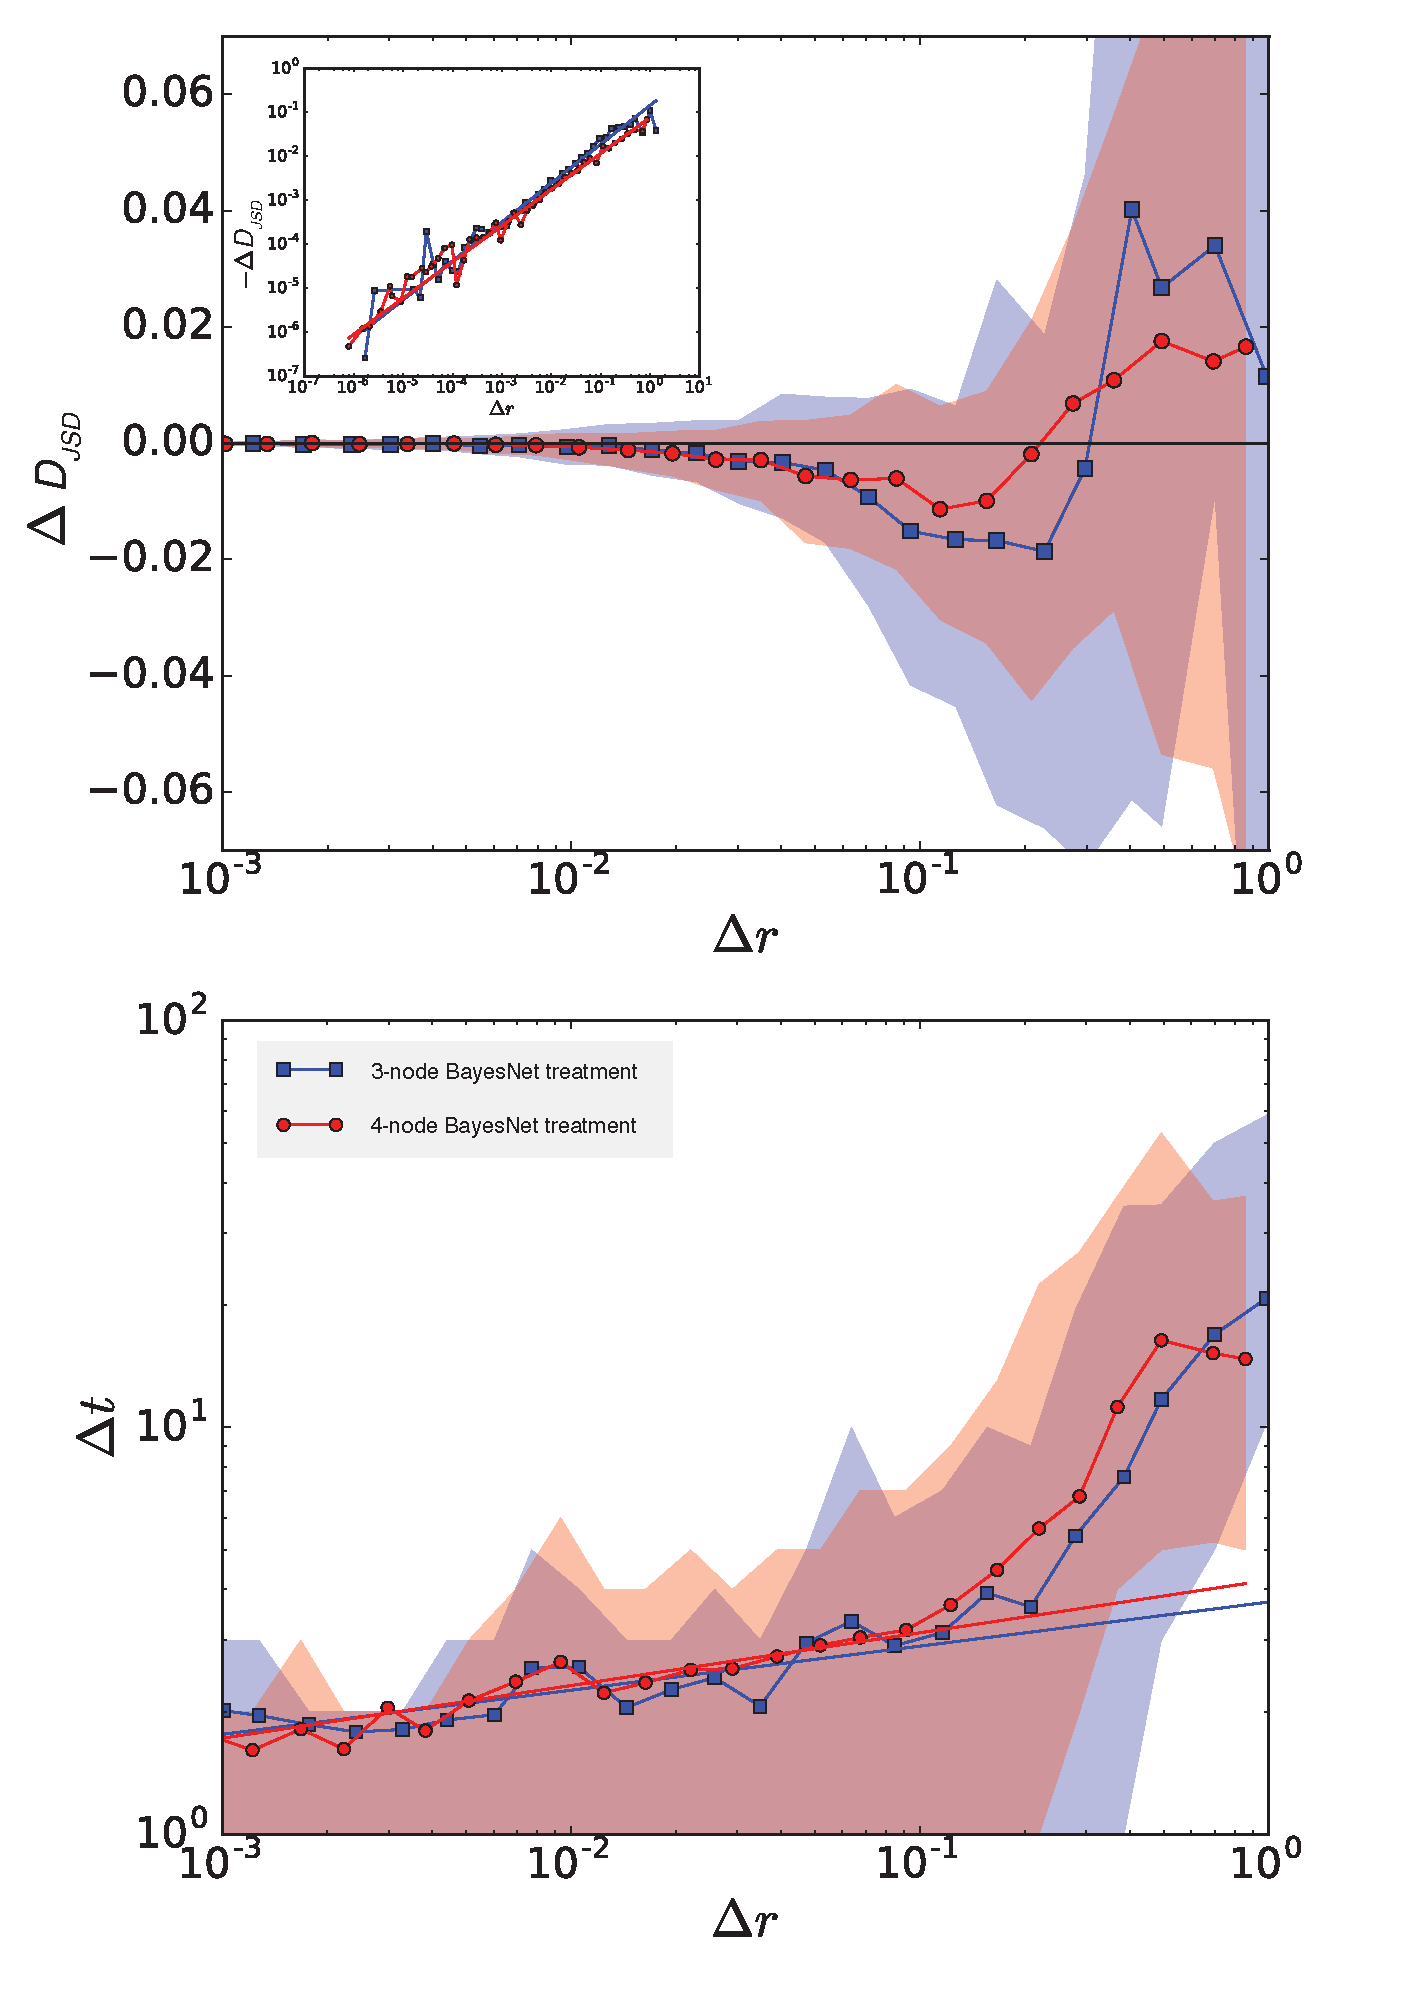
\includegraphics[width=11cm]{figures/vs_dr.eps}
\caption{{\bf A.} Evolution of the distance to the true model $D$ as a function of displacement $\Delta r$. The distance scales as $D \sim {\Delta r}^{\mu}$ with $\mu_{simple} = 0.88(1)$ [resp. $\mu_{complex} = 082(2)$]. For $\Delta r > 0.2$, $D$ becomes quickly highly uncertain, but rather positive, reflecting the {\it cost} of the making ``wild"displacements. {\bf B} For $\Delta r < 0.2$, the waiting time before a displacement decision is made scales as $\Delta t \sim \Delta r^{\gamma}$ with $\gamma_{simple} = 0.11(1)$ [resp. $\gamma_{complex} = 0.13(1)$]. For $\Delta r > 0.2$, the waiting time before a displacement decision is taken get disproportionally long (up to tens of seconds on average for displacement of 0.7 (i.e., $\approx 25\%$ of the maximum displacement distance). On both panels, blue and red areas show the 25th percentile confidence intervals.}.
%\caption{Scaling relation between $\Delta t$ and $\Delta r$ for the simple (A) and complex (B) treatments. The functions are similar for both treatments [resp. $\sim 0.44(2)$ ($p < 0.01$ , $r = 0.39$) and $\sim 0.47(2)$ ($p < 0.01$ , $r = 0.36$)]. {\bf Actually, one may see this figure differently : scaling $\Delta t \sim {\Delta r}^{0.2}$ for $\Delta r < 0.2$ and another (unknown) regime for $\Delta r > 0.2$ with waiting time getting disproportionately long $\rightarrow$ This may highlight the processing costs associated with a big jump.}}
\label{fig:vs_dr}
\end{center}
\end{figure}




%\section{Model of L\'evy Walks/Flights in cognition, incorporating memory}


\begin{figure}[h!]
\begin{center}
\includegraphics[width=10cm]{figures/schematic_displacement.eps}
\caption{\footnotesize{2-dimensional schematic description of the {\it L\'evy flying mind} model ({\bf ``Proportional Attraction"}): At each time step, the individual must choose between remaining in the solution envelope that has already been explored and exploring outside the currently known solution envelope.  We assign some probability $p$ (a number between 0 and 1) to the participant's decision of staying in the explored envelop and probability $1-p$ to the decision to explore outside that envelop.  If it is harder to find solutions that offer a balanced re-combination of previous solutions than to think out-of-the-box and propose solutions outside of the current solution envelope, then $p < \frac{1}{2}$ else $p \geq \frac{1}{2}$.}}
\label{fig:schematic}
\end{center}
\end{figure}

%\section{What can we learn from stylised facts regarding timing ?}

%\section{Discrete cascading models and recombination of knowledge}




\section{Discussion}

Outstanding problems :

- decreasing mean square displacement: it basically seems that with time displacement decreases: This can be due to (i) the limited space (unlikely), (ii) some convergence toward the true model, or (iii) some stickiness, or (iv) probably (ii) and (iii) together.
  
- connecting cascades and memory with (i) evolutionary theory and (ii) increased success (resp. counter-performance). Connect also with potential cascading processes in cognition (any knowledge about this? memory?)

- time between return visits (if return visits happen in close time, then it matters little)

- connect results with Distance Decay, but basically a model could be summarized as $Distance \sim S_T$ (by the way $D_{min}$ versus $S_T$ could be improved by looking at $D_t$ versus $S_t$). $S_T$ (resp. $S_t$) is a function of displacement $\Delta r$ decisions (which may also cost additional time) and (obviously) their influence on score. 

In summary, there is at some point a displacement decision with a part of ``risk", which can by the way be discounted by time spent (waiting time relative to avg waiting time and/or experimentation duration and/or time left). Large displacement can be associated with more risky exploration and more time required for decision. It looks like there is a $\Delta r$ which maximize improvement ($\Delta r \approx 0.15$). This is interesting because it suggests that such move size maximizes the chance that a new patch will be visited.


potential long reach :

- qualitative/quantitative differences between performing/non-performing participants?













\input{sections/conclusion}

\clearpage
%\section*{Methods}
\subsection*{Subjects, Experiment, Treatments and Compensation}
We recruited 96 subjects ($n_{female} = ??$, $n_{male} = ??$) on Columbian University campus. The experiment took place at the social science laboratory (IRB approval : ???). Upon arrival, subjects were briefed and directed to an individual booth . The experiment was performed on a graphical  html/javascript interactive Web interface. All actions taken on the interface by subjects were recorded in real-time (resolution : $1s$). Subjects were asked to reverse-engineer the causal structure and the probabilistic relationships between nodes of an acyclic directed graph (i.e., Bayesian network). There were 2 treatments with respectively 3 and 4 nodes and their causal relationships. Participants were enabled to dynamically update their models. Participants were compensated according to their predictions and their predictions' congruence with a series of realizations.  The incentives to make good predictions were determined according to the Becker-DeGroot-Marschak method \cite{becker1964measuring}. {\bf  [The method implies a quadratic loss function.]} (See SI \ref{SI_experiment})


\bibliographystyle{apsrev4-1}
\bibliography{bib/references,bib/cognition_causality,bib/levyflight_foraging,bib/misc,bib/orgsci}

\clearpage
%

\section{Experiment}
\label{si:experiment}

\section{Jump Sizes $\Delta r$}

Euclidean distance : 

\begin{equation}
\Delta r = d(p, q) = \sqrt{(p_1- q_1)^2 + (p_2 - q_2)^2+\cdots+(p_i - q_i)^2+\cdots+(p_n - q_n)^2}.
\end{equation}

with $n=8$ (3-nodes BayesNet) or $n=16$ (4-npdes BayesNet) and $p$,$q$, 2 consecutive position vectors

\begin{figure}[h!]
\begin{center}
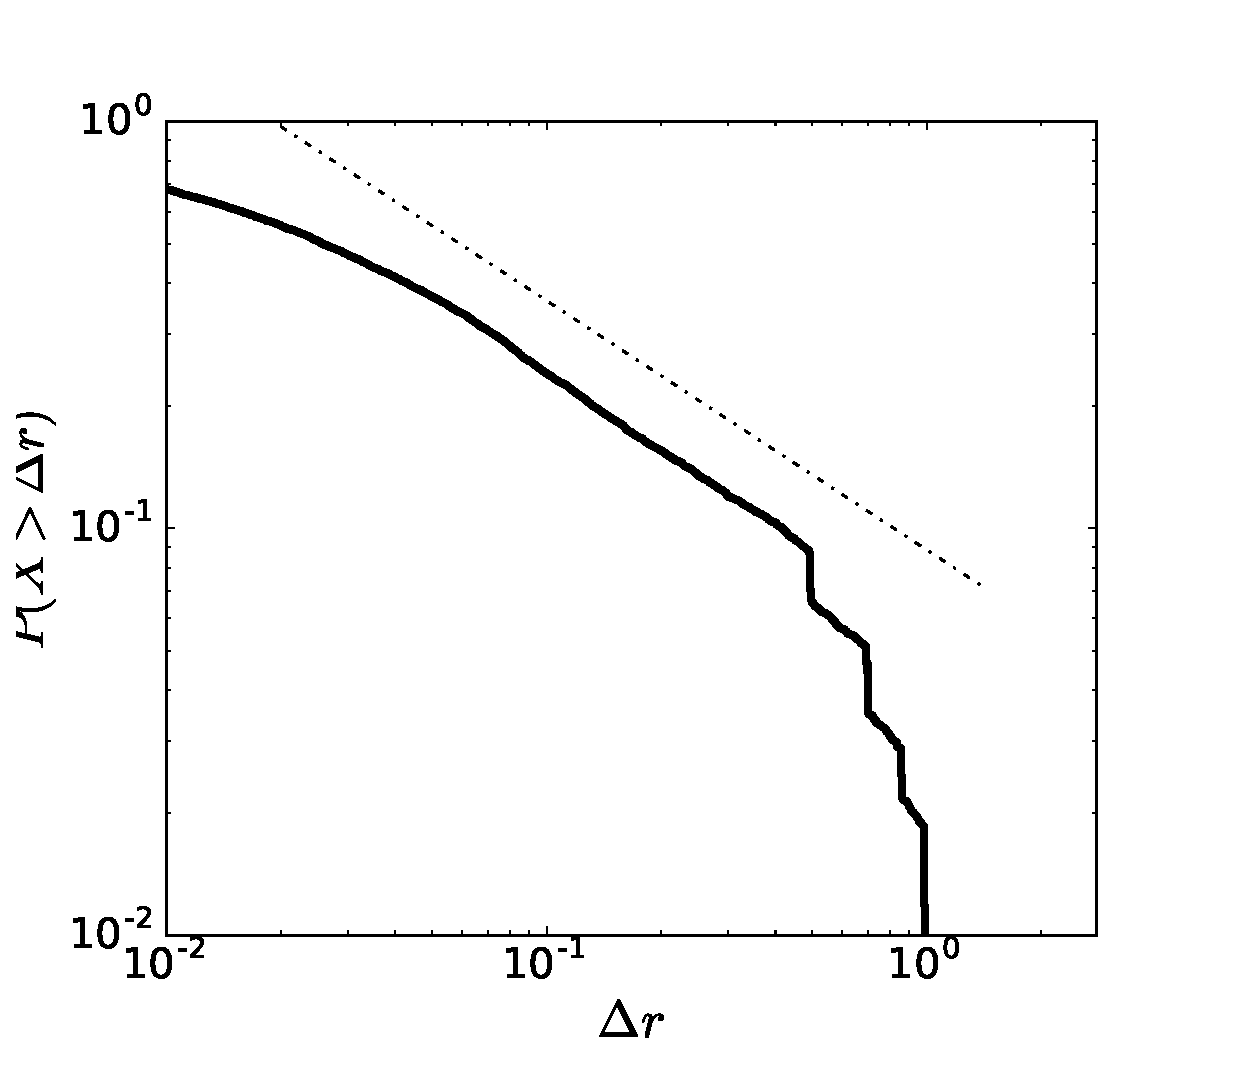
\includegraphics[width=10cm]{figures/CCDF_Displacement_simple.eps}
\caption{(3-node BayesNet) : exponent $\alpha = 0.61(3)$ with upper cutoff  $x_{max} \approx 1.4$ (theoretical limit is $x_{max} = 2\sqrt{2}$).}
\label{fig:jump_sizes}
\end{center}
\end{figure}


\section{Waiting Times $\Delta t$}



\begin{figure}[h!]
\begin{center}
\includegraphics[width=15cm]{figures/dt_kernel_SI.eps}
\caption{Distribution of Waiting Times (fitted by kernel density estimators \cite{}) exhibits a change of regime typical of changes of regimes in waiting times \cite{maillart2011,saichevTheory}: $\beta_{\Delta t  \leqslant 100} \approx 0.46(3)$ (slope $\sim t^{-(1+ \beta_{\Delta t  \leqslant 100})}$ represented by dashed line) and $\beta_{\Delta t > 100} \approx 1.65(1)$ (slope $\sim t^{-(1+ \beta_{\Delta t  > 100})}$ represented by continuous line).}
\label{fig:waiting_times}
\end{center}
\end{figure}


\section{Correlation $\Delta r$ and $\Delta t$}
\label{si:corr_dr_dt}


\begin{figure}[h!]
\begin{center}
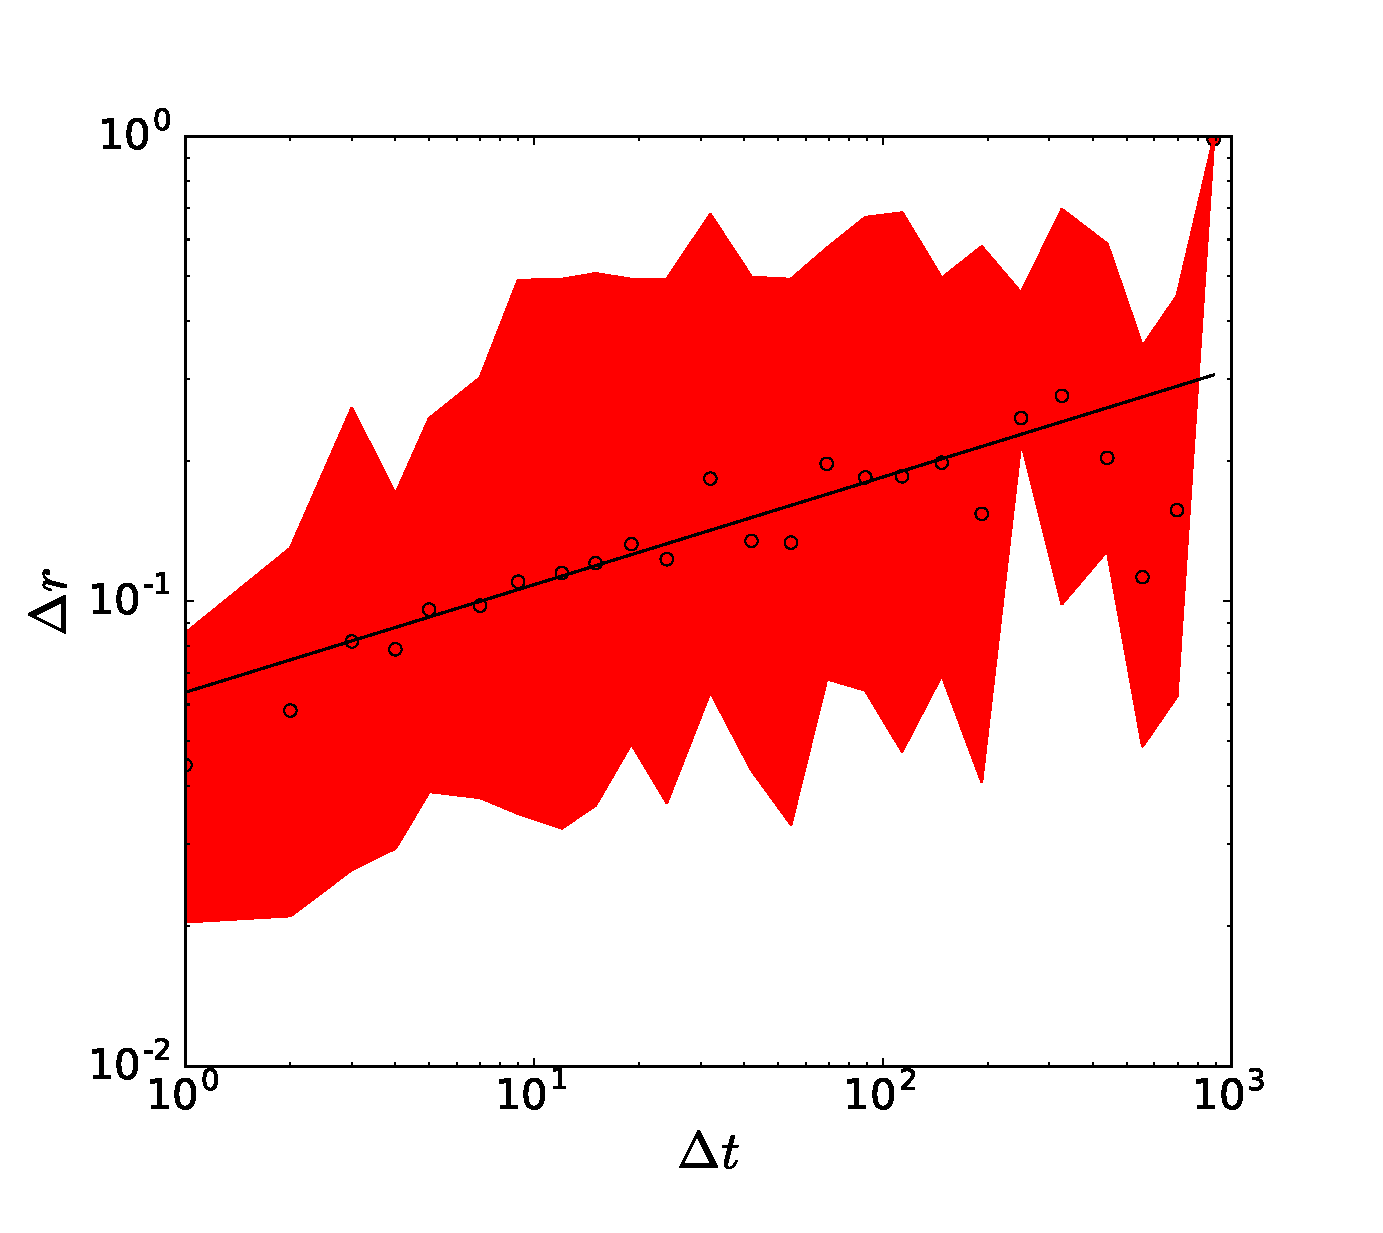
\includegraphics[width=10cm]{figures/cor_Delta_t_Delta_r_simple.eps}
\caption{3-node BayesNet : Correlation (Spearman rank correlation) between $corr(\Delta r,\Delta t) \approx 0.32$, and the main direction of dependence can be approximated by a scaling function $\Delta r \sim {(\Delta t)}^{0.23(2)}$ (least square fit of values in double logarithmique scale, $p < 0.001$ and $R= 0.21$}
\label{fig:corr_dr_dt}
\end{center}
\end{figure}






%\renewcommand\thesection{\Alph{section}}
\renewcommand\thesection{S\arabic{section}}
\setcounter{section}{0}

\renewcommand\theequation{S\arabic{equation}}
\setcounter{equation}{0}


%\begin{center}
%{\Large Supplementary Information}
%\vspace{3 cm}
%\end{center}

%

\section{Experiment}
\label{si:experiment}

\section{Jump Sizes $\Delta r$}

Euclidean distance : 

\begin{equation}
\Delta r = d(p, q) = \sqrt{(p_1- q_1)^2 + (p_2 - q_2)^2+\cdots+(p_i - q_i)^2+\cdots+(p_n - q_n)^2}.
\end{equation}

with $n=8$ (3-nodes BayesNet) or $n=16$ (4-npdes BayesNet) and $p$,$q$, 2 consecutive position vectors

\begin{figure}[h!]
\begin{center}
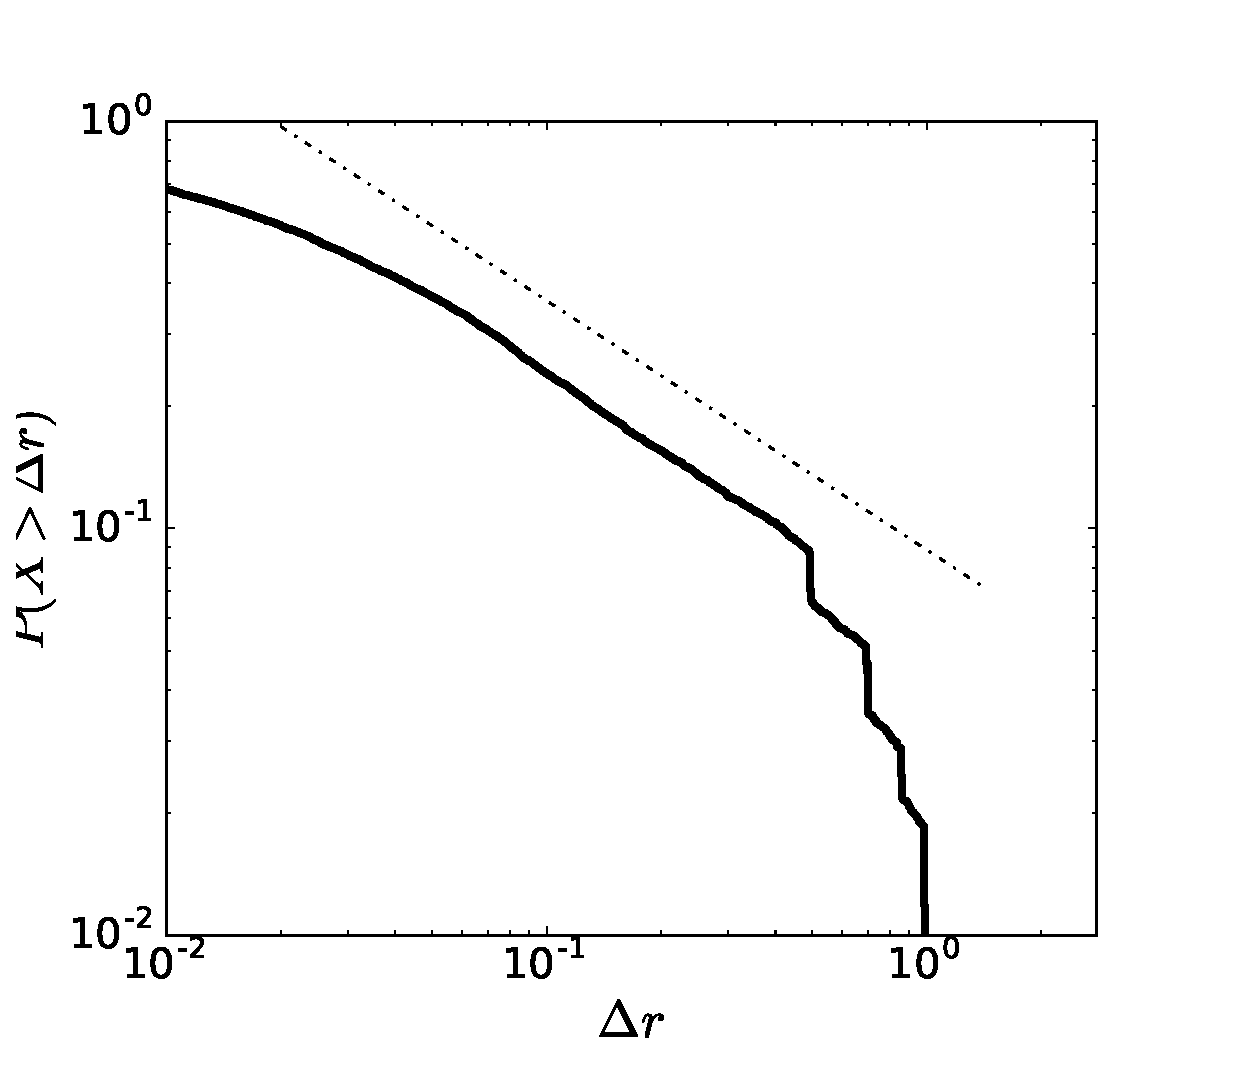
\includegraphics[width=10cm]{figures/CCDF_Displacement_simple.eps}
\caption{(3-node BayesNet) : exponent $\alpha = 0.61(3)$ with upper cutoff  $x_{max} \approx 1.4$ (theoretical limit is $x_{max} = 2\sqrt{2}$).}
\label{fig:jump_sizes}
\end{center}
\end{figure}


\section{Waiting Times $\Delta t$}



\begin{figure}[h!]
\begin{center}
\includegraphics[width=15cm]{figures/dt_kernel_SI.eps}
\caption{Distribution of Waiting Times (fitted by kernel density estimators \cite{}) exhibits a change of regime typical of changes of regimes in waiting times \cite{maillart2011,saichevTheory}: $\beta_{\Delta t  \leqslant 100} \approx 0.46(3)$ (slope $\sim t^{-(1+ \beta_{\Delta t  \leqslant 100})}$ represented by dashed line) and $\beta_{\Delta t > 100} \approx 1.65(1)$ (slope $\sim t^{-(1+ \beta_{\Delta t  > 100})}$ represented by continuous line).}
\label{fig:waiting_times}
\end{center}
\end{figure}


\section{Correlation $\Delta r$ and $\Delta t$}
\label{si:corr_dr_dt}


\begin{figure}[h!]
\begin{center}
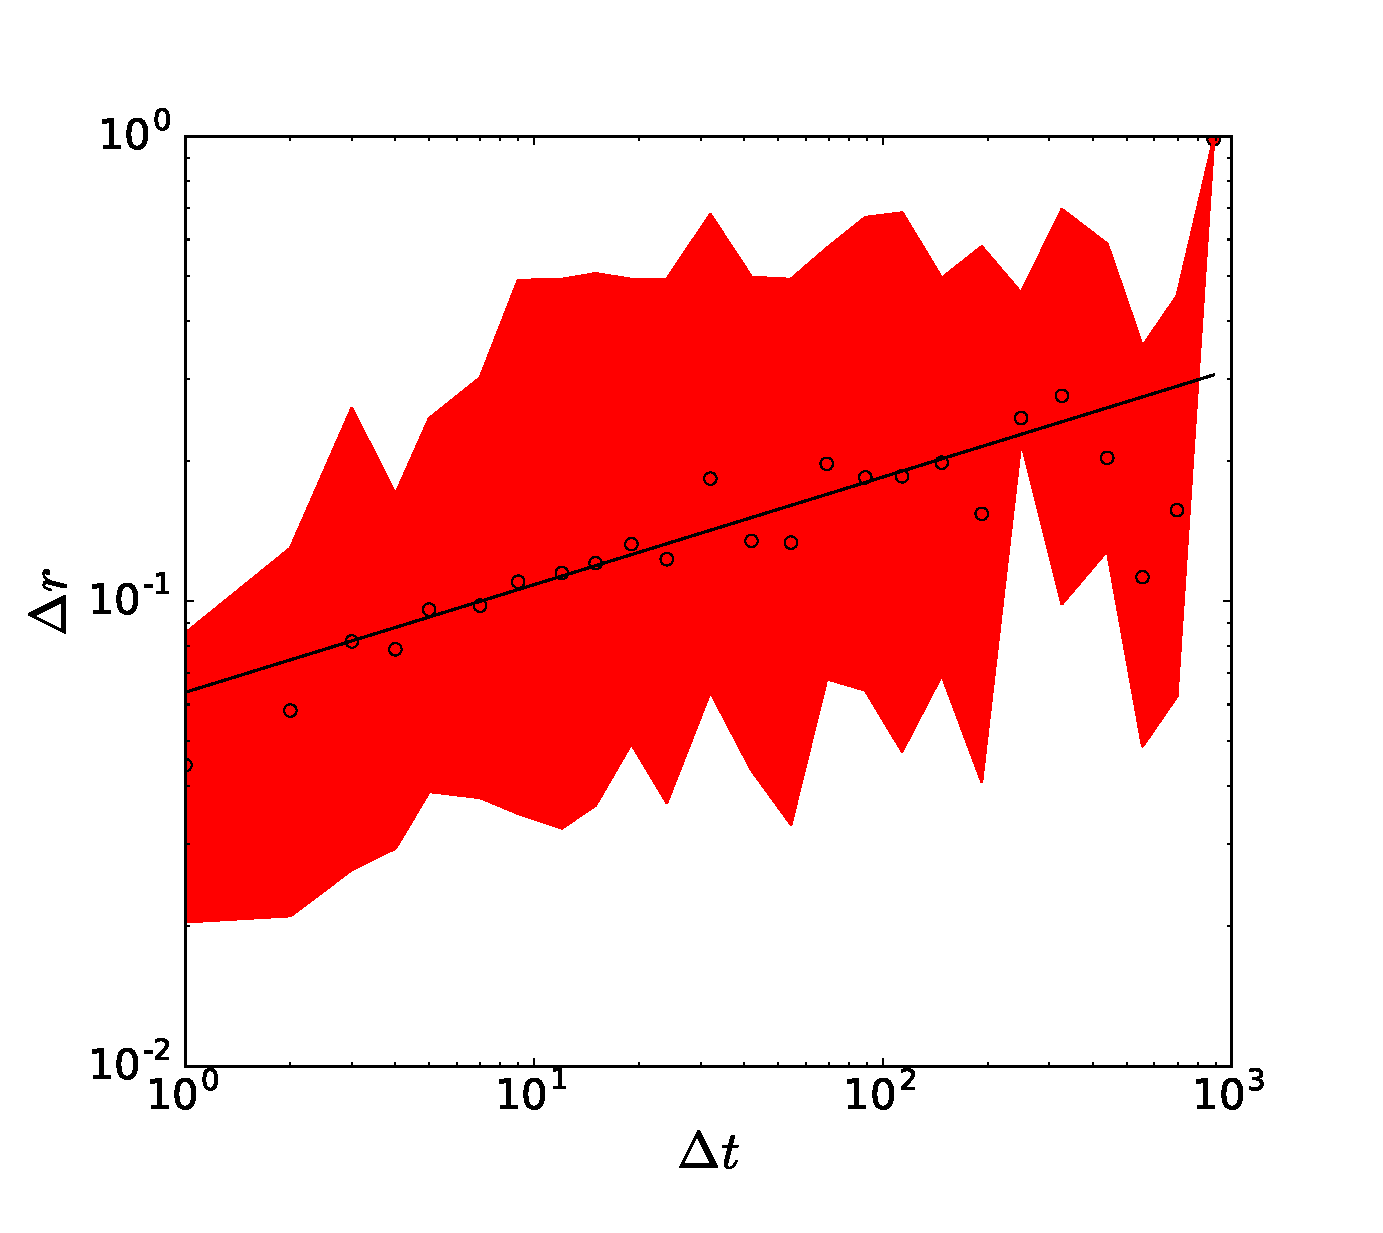
\includegraphics[width=10cm]{figures/cor_Delta_t_Delta_r_simple.eps}
\caption{3-node BayesNet : Correlation (Spearman rank correlation) between $corr(\Delta r,\Delta t) \approx 0.32$, and the main direction of dependence can be approximated by a scaling function $\Delta r \sim {(\Delta t)}^{0.23(2)}$ (least square fit of values in double logarithmique scale, $p < 0.001$ and $R= 0.21$}
\label{fig:corr_dr_dt}
\end{center}
\end{figure}





%\section{Literature Review}
The cognitive science and economics literatures have found much evidence in support of consistency with as well as deviance from human learning with Bayesian constructs of learning. On average, especially when incentives are high and tasks extremely simple, subjects update their beliefs based on new data in a way that is consistent with Bayes rule. However, at the individual level, there are large variations, as well as systematic departures under certain conditions.  In these literatures, comparing human learning to Bayesian updating, observed deviations can be organized in terms of "biases" or "heuristics".  Deterministic bias may have the consequence of underweighting or overweighting evidence ('law of small numbers' ) relative to base rates.  Such biases are in turn explained by the concept of availability heuristic (Griffin and Tversky 1992), which reduces data to examples that immediately come to mind, rather than by considering the exhaustive data of all previous experience and it has the consequence of slowing learning.  An example of the latter is recency bias \citep{FudenbergPeysakhovich2014}.  Another obstacle to efficient learning is when ambiguous information is taken to be a confirmation of a currently held hypothesis, or when information is suboptimally acquired or remembered.  Additionally, people have been found having difficulties with contingent reasoning with regards to future events \citep{CharnessLevin2009}. 
 
A different literature, associated with many disparate disciplines, such as ecology, cognitive science and complex systems frames learning and behavior in uncertain environments in terms of search, a ubiquitous property of life (Hills, Thomas T. et al. 2015).  Search, in turn, is a process of exploration and exploitation.  If behavior remains stable over some period of time, is focused and stays within a narrow subspace of the feasible decision or belief space it is interpreted as exploitation.  If it is erratic and moves wildly, it is interpreted as exploration (Mehlhorn et al, 2015).   

%These departures are clues to the heuristics humans use in their judgments, which overall often approximate bayesian inference but are not equivalent. Although many of these deviations imply that learning should be slower than predicted by Bayes rule,  few experiments measure the rate of learning and how far it departs from Bayesian inference.  

But why should one search and not simply count past events as Bayesian and Frequentist rationality demand (co-occurrences of values of a set of variables)?  With regards to counting observed frequencies of co-occurrences in order to measure covariances between a set of variables, if the number of variables gets large, the number of possible co-occurrences becomes astronomical.  Thus, remembering how many times a particular constellation of values of a given set of variables co-occurred puts ever increasing demands on memory as the set of variables gets large.  "In any system responsible for managing a vast data base there must be failures of retrieval" (Anderson, J. R., & Schooler, L. J. 1991).  Hence optimality must not mean Bayesian or Frequentist optimality, as counting all possible co-occurrences is not feasible because of limits on memory.  Additionally, there is the problem of assigning beliefs to never before experienced co-occurrences.  Note that Anderson, J. R., & Schooler, L. J. 1991 present not an argument about specific human biases or heuristics but rather one that presupposes a different definition of optimality that takes natural limits into consideration.  Our work begins with this same definitional premiss.  In addition to their own findings, Anderson, J. R., & Schooler, L. J. 1991 review the pervasive findings of power functions in the learning literature with respect to positive and negative performance measures and time.  As long as the performance measure is either unbounded or does not approach its bounds, the relationship between performance and time seems to follow the functional form:
$$P = A*T^{b},$$
where $b$ is negative and $P$ can either have negative valence, such as number of trials necessary to learn someone's name, or positive valence such as probability of having retained a name. In our case, the measure is bounded, above by 1 and below by 0, but never approaches either of its bounds. 

Learning of statistical systems can also be seen as search processes in simplex-spaces. If we consider learning as searching with feedback and we may do so if we find that brains learn as brains search, then another literature becoomes relevant that has not been generally considered by those studying learning; the literature concerened with foraging and the sort of spacial learning that had been most relevant throughout human evolution.  For most of our evolutionary history there were no stock and insurance markets and thus there is no reason to believe that our brains were optimized for the sort of learning that is optimal in those modern scenarios.      
%We find that it is not (slower). Furthermore, we also find that the quality of the inferences at each time space and across players varies a lot, following a "punctuated equilibrium" pattern. These observations are thus additional clues about the cognitive processes at play, with fine-grained information about how subjects update their beliefs in response to new information and the success and failure of their bets. Below were review some of the promising cognitive mechanisms posited to explain some of the deviations above and which can be evaluated in light of our data.

%2) Cognitive mechanisms 
%Interesting mechanisms have to do with how people organize the hypothesis space and sample from it. 
%- sampling hypothesis
%- change of paradigm when observing "surprising events" (Ortoleva)

%the satisficing principle may also mediate the learning process because computations such as bayes rules are costly. 

%\section{Problem Formulation}
\subsection{Intuition}

Random search processes occur in many areas, from the foraging behavior of bacteria and animals \cite{}, to human mobility \cite{}, to computer search and optimization algorithms \cite{}.  When searching for solutions to outstanding problems, humans must come up with innovative solutions, which involve random search (e.g., gathering information, etc), along with the consolidation of past and current experience.

Here, we show how people go through the resolution of a complicated problem, starting from no knowledge through L'evy random search, involving synthesizing current knowledge versus exploring out-of-the box (see Figure \ref{fig:schematic}). We then measure how this process leads to convergence, albeit very slow convergence, to the solution.

%{\bf huge mistake?:  the displacement is not necessarily the path to a better solution. JS-Distance is a by-product of displacement (of the search process) $\rightarrow$ JSD is the objective function NOT the process}

\subsection{Simple case}

The intuition is that large jumps lead to super-diffusion while long-waiting times lead to sub-diffusion. Here, we see both large jumps and long waiting times. There is thus a tension between the two factors and how they respectively influence the random search process. However, both are correlated: larger waiting times lead to larger jumps, yet with a decreasing marginal function ($\Delta r \sim {(\Delta t)}^{\nu},~with ~\nu \approx 0.23 < 1$). This suggests that waiting times may trigger more aging (sub-diffusion), compared to long-range search (i.e., super-diffusion), which has been found to be an optimal search \cite{optimal_random_search}. 




\subsubsection{Jump size}

\be
P(\Delta r) \sim r^{-(1+\alpha)},~with~\alpha = 0.61(3).
\ee

with upper cut-off $max(\Delta r) \approx 1$ close to the absolute max ($2\sqrt{2} \approx 2.83$).

\subsubsection{waiting times}

\be
P(\Delta t) \sim t^{-(1+\beta)},~with~\beta = 0.46(3).
\ee

with a change of regime for $\Delta t > 100$ (in that case: $\beta = 1.65(1)$).

\subsubsection{Dependence between $\Delta r$ and $\Delta t$}

nb: We find a dependence (Spearman rank correlation $corr = 0.32$) between  $\Delta r$ and $\Delta t$, which can be approximated by

\be
\Delta r \sim {(\Delta t)}^{\nu},~with ~\nu = 0.23(2)
\ee


\subsubsection{mean square displacement}

\be
MSD = \langle r(t)^2 \rangle = t^{\gamma},~with~\gamma = 0.35(1).
\ee

$\rightarrow$ subdiffusion

\subsubsection{Number of distinct locations visited}

\be
S(t) \sim t^{\mu},~with~\mu = 0.85(0)
\ee

\begin{center}
\ba
\Delta S / \langle S \rangle = S^{0.33(2)}\\
%\ee
~or~\\
%\be
\Delta S / \langle S \rangle = e^{-\lambda S},~with~\lambda = 1.6\times 10^{-2}
\ea
\end{center}



\clearpage



\subsection{Jensen-Shannon Distance}


\begin{equation}
{\rm JSD}(P \parallel Q)= \sqrt{\frac{1}{2}D(P \parallel M)+\frac{1}{2}D(Q \parallel M)}
\end{equation}
where $M=\frac{1}{2}(P+Q)$


The Jensen-Shannon Distance (JSD) is a measure of mutual information. We use it to compare the distance of a Bayes Net model from the truth (see Figure \ref{fig:decay}), and between models.\\


Score:
\begin{equation}
S = 1 - JSD
\end{equation}



\subsection{Ultra Slow Diffusion / Power Law Decay}

The CTRW model predicts that the mean square displacement (MSD) asymptotically follows $\langle \Delta x^2 (t) \rangle \sim t^{\nu}$ with $\nu = 2\beta /\alpha$

\begin{equation}
\label{power_law_decay}
JSD(t) = C \cdot t^{-\alpha},
\end{equation}

with $\alpha = 0.09$ and $C$ a constant, specific to the $simple$ and $complex$ models

\begin{equation}
\label{ultraslowdiffusion}
S(t) = 1 - JSD(t) = 1- C \cdot t^{-\alpha},
\end{equation}


\subsubsection{Stepwise Jumps}

\begin{equation}
P(R > \Delta r) \sim |\Delta r|^{-\alpha}, ~~with~~\alpha \approx 0.1,
\end{equation}

jump size $\Delta r$ Figure \ref{fig:jump_sizes}



\subsubsection{Memory Effects / Waiting Times}

waiting time $\Delta t$


Figure \ref{fig:waiting_times}

\begin{equation}
P(T > \Delta t) \sim |\Delta t|^{-\beta}, ~~ with~~  1< \beta < 2
\end{equation}



\subsubsection{Continuous Time Random Walk (CTRW)}

continuous-time random walk (CTRW)  $\rightarrow$ is a generalization of a random walk where the wandering particle waits for a random time between jumps. It is a stochastic jump process with arbitrary distributions of jump lengths and waiting times.[1][2][3] More generally it can be seen to be a special case of a Markov renewal process.

\begin{equation}
\psi(\Delta r,\Delta t)=P(\Delta r)P(\Delta t)
\end{equation}

with $P(\Delta r)$ and $P(\Delta t)$ are not dependent.

{\bf Jump length pdf :}
\begin{equation}
\lambda(\Delta r) = \int_0^{\infty} dt \psi(\Delta r,\Delta t)
\end{equation}

{\bf Waiting Time pdf :}
\begin{equation}
w(\Delta t) = \int_{-\infty}^{\infty} dx \psi(\Delta r,\Delta t)
\end{equation}

Characteristic waiting time:
\begin{equation}
T \int_0^{\infty} dt w(t)t
\end{equation}


Characteristic waiting time:
\begin{equation}
\Sigma^2 = \int_{-\infty}^{\infty} dx \lambda(x) x^2
\end{equation}


\subsection{Number of distinct locations / Visitation frequency:}

(A) The number of distinct locations $S(t)$ visited by a randomly
moving object is expected to follow:


\begin{equation}
S(t) \sim t^{\mu}
\end{equation}


where $\mu = 1$ for LŽvy flights [24] and $\mu = \beta$ for CTRW. {\bf [Here, it is unclear what visiting a distinct location means ]}
The probability $f$ of a user to visit a given location is expected to be asymptotically uniforma ($f\sim const.$) for both LŽvy flights and CTRWs. In contrast, the visitation patterns of humans is rather uneven, so that the frequency $f$ of the $k$th  most visited location follows

\begin{equation}
f_k ~k^{-\zeta}
\end{equation}

where $\zeta \approx 1.2 \pm 0.1$ (babarasi paper).


\subsection{slight anisotropy}
The propagator is anisotropic: There is equal chance that a jump will be negative or positive. However, the distribution of jump size is different: both are power law, but with different exponents.

isotropy :
\begin{equation}
W_j (t+\Delta t) = a W_{j-1}(t) + b W_{j+1}(t)
\end{equation}

with $a=b=1/2$. In case of anisotropy $\rightarrow  a \neq b$.



\subsection{Exploration versus Exploitation}
Each new BayesNet iteration may be a combination of former iterations, or rather something new. It is difficult to determine if {\it exploration} occurs, by opposition to {\it exploitation}. The intuition is that if the sum of distances between the new node and all existing nodes (weighted by their iteration number) is larger than at the previous step, then more exploration occurs

\begin{equation}
\overline{JSD}(N) =  \sum_{n=0}^{N-1} \frac{JSD(n,N)}{n}
\end{equation}



\subsection{Formulation of reuse, with memory}

%\section{Measures of Cognitive Distance}

In this section, we will introduce various measures.  We use the square root of a measure called the Jensen Shannon Divergence as our measure of cognitive distance (CD). The performance score is then

\begin{equation}
S = 1 - CD.
\end{equation}

In order to understand the usefulness and reason behind this measure this section introduces some preliminary measures which the Jensen-Shannon Divergence builds on and then formally defines our measure of cognitive distance.    
  
\subsection{The Shannon Entropy}

An important measure of ignorance is the Shannon Entropy, which is maximized whenever all possible events are believed to occur with equal probability:

$H(X)=-\sum_ip_i(x_i)\log(p_i(x_i)).$

The entropy of a stochasic process, $\{X_i\}$ is defined by 

$H(\chi)=\lim_{n\rightarrow\inf}\frac{1}{n}H(X_1, \ldots, X_n),$

when the limit exists, which in this case it does as it was picked by us. 
We can calculate, then, that the Shannon Entropy of the simple ``treatment'' system is $2.7$ and that of the complex one is $3.26$. However, distributions over larger alphabets tend to have higher entropy and for our purposes the entropy should be considered a relative measure over distributions of the same cardinality. 

Specifically, the maximum entropy for categorical variables with $N$ categories is $\log_2(N)$, which happens when for each category, $x_i$, its probability is $p_i(x_i)=\frac{1}{N}$. 

This fact can be appreciated on hand of a mental or computational experiment \citep{Cover13} where there is an automatic type writer that randomly prints a sequence of letters from an alphabet with $m$ members, where at each time, $t$, each member of the alphabet has an equal chance of $\frac{1}{m}$ to be chosen as the next member of the sequence. The type writer can produce $m^t$ possible sequences of length $t$, each of them as likely as any other. We then have that 

$H(X_1, \ldots, X_t)=\log(m^n)$ and the entropy rate is $H(\chi)=\log m$ bits per symbol. 

In the current case, we can substitute $m$ with the number of possible combinations (joint states) that $k$ binary variables can assume: $2^k$.
The simple system has $k=3$ binary variables and its maximum entropy (random type writer) belief has entropy $\log_2(N)=\log_2(2^k) = 3$. The more complex treatment system has $k=4$ binary variables and thus its maximum entropy belief has entropy $\log_2(N) = 4$. Entropy is also always positive, so that the measure is bounded between $0$ and the logarithm of the number of joint states $2^k$ that define the system. The Shannon Entropy is measured in bits when the base $2$ logarithm is used and it can be interpreted as the average number of yes or no questions a person needs to ask someone who knows the current outcome in order to gain knowledge of it.  In the worst case, this requires as many yes or no (high, or low) questions as there are binary variables, $k$. 

\begin{figure}
\noindent\makebox[\textwidth]{%      
        \includegraphics[width=1\textwidth]{figures/simplejoint.png}}
\caption{The limiting distribution of the simple treatment and an example frequency distribution pertaining to 400 random realizations.}
\label{fig:simplejoint} 
\end{figure}

But it is easy to see from a picture of the joint distribution describing joint behavior of the simple system (Figure \ref{fig:simplejoint}), for example, that very often three questions won't be needed. We could ask the person who knows whether the first variable, labeled ``Financial Sector'', has taken on the value ``H''.  If the answer is no, we could ask if the outcome is the event ``L'', ``H'', ``L'' and very often we would be right, finding the answer with only $2$ yes or no questions. Better yet, if we knew or somehow guessed the correct causal structure, we would know that whenever the ``Financial Sector'' variable takes on the value ``L'' and the ``Interest Rate'' variable assumes the value ``H'', the ``Industry'' variable must be in the low state. So, if we asked first ``is the value of the Financial Sector high'' and received ``no'' as an answer and then we asked ``is the value of the Interest Rate high'' and we received ``yes'' as an answer, we could be certain that the outcome must be ``LHL''. On average, for the simple system we would need to ask $2.7$ yes or no questions, if we know the distribution.   

\subsection{The Kullback-Leibler divergence}

The Kullback-Leiber Divergence was proposed as a measure of difference between two probability distributions $P$ and $Q$. Specifically, it was meant as a measure of the information that is lost when belief $Q$ is used as an approximation for a true probability distribution $P$:
\\

$D_{KL}(P(X) | | Q(X))=\sum_ip_i\log_2(\frac{p_i}{q_i}).$
\\

It is readily apparent that the Kullback-Leibler divergence can be re-expressed as follows:
\\

$D_{KL}(P(X) | | Q(X))=\sum_i (p_i\log_2p_i -p_i\log_2q_i = H(P, Q)-H(P)$, 
\\

where $H(P, Q)$ is known as the cross-entropy of $P$ and $Q$, and $H(P)$ is simply the entropy of $P$.

There are two problems with the Kullback-Leibler divergence as a measure of distance: 1) it is not symmetric ($D_{KL}(P | | Q) \not= D_{KL}(Q | | P)$) and 2) for the two distributions $P$ and $Q$, if one of the $q_i$ is equal to $0$, but the corresponding $p_i$ is not equal to $0$, the measure is not defined.  For example, we can see that when we simulated the complex process, some of the theoretically rare but possible outcomes have not yet occurred during the simulation and thus, if we want to measure the distance between the theoretical distribution and the frequencies of the simulated outcomes, using the Kullback-Leibler divergence, we will find that this measure is not defined. 

\subsection{The Jensen–Shannon divergence}

The Jensen–Shannon divergence is a symmetrized version of the Kullback-Leibler divergence that also solves the zero division problem:
\\

$D_{JS}(P | | Q)=\lambda*D_{KL}(P | | M) + (1-\lambda)*D_{KL}(Q | |M),$ 
\\

where $M=\lambda P + (1-\lambda) Q$ and $\lambda$ is usually, but not necessarily equal to $\frac{1}{2}$. In order for the measure to be symmetric, $\lambda$ has to be equal to $\frac{1}{2}$. 


The value of the Jensen-Shannon divergence is always between $0$ and $1$; $0$, when the two distributions are the same and $1$ when the two distributions have orthogonal support. This measure quantifies the amount of information in bits, about which of the two distributions one bit of data was drawn from, given that it was drawn from the first distribution with probability $\lambda$ and from the second with probability $1-\lambda$. For example, if the two distributions are the same, any bit of data will render no information about which of the two identical distributions it was drawn from, while if the two distributions have orthogonal support, each bit of data gives exactly one bit of information. To state this in Bayesian terms: if the two distributions are the same, then we can not learn from data and our posterior probability about which of the two distribution that data was drawn from is equal to our prior ($\lambda$ for the first distribution). At the other extreme, if the distributions have orthogonal support, the posterior will put probability $1$ on the distribution that supports the data; one bit of data carries one bit of information. 

\subsection{Cognitive Distance and the Performance Score}

If the square-root of the Jensen-Shannon divergence is taken, the result is a metric known as the Jensen-Shannon distance. This is the distance metric we use to calculate distances between any two distributions.  We refer to it as Cognitive Distance (CD):

\begin{equation}
CD(P, Q) = \sqrt{D_{JS}(P | | Q)}
\end{equation}

and to remind the reader, our performance score of person $i$ at time $t$, (supressing the index $i$), $S_t$, is 

\begin{equation}
S_t = 1 - CD(M_t, T),
\end{equation}

where $M_t$ is some person's Bayes Net model, at time $t$, of the true stochastic system, $T$. 


\end{document}




 


